% lecture7.tex -- GENERATED by build_L7.py from L7_numbers.json; do not edit by hand.
\documentclass[10pt,aspectratio=169,t]{beamer}
% =============================================================================
% emqa_preamble.tex -- shared Beamer preamble of Energy Markets Quantitative Analysis (EMQA)
% Used by every lecture: lectures/Lk/lecturek.tex does
%   \documentclass[10pt,aspectratio=169,t]{beamer}
%   % =============================================================================
% emqa_preamble.tex -- shared Beamer preamble of Energy Markets Quantitative Analysis (EMQA)
% Used by every lecture: lectures/Lk/lecturek.tex does
%   \documentclass[10pt,aspectratio=169,t]{beamer}
%   % =============================================================================
% emqa_preamble.tex -- shared Beamer preamble of Energy Markets Quantitative Analysis (EMQA)
% Used by every lecture: lectures/Lk/lecturek.tex does
%   \documentclass[10pt,aspectratio=169,t]{beamer}
%   \input{../common/emqa_preamble}
%   \emqalecture{k}{Lecture title}
% Logos live in lectures/common/logos/, charts in lectures/Lk/charts/.
% Do NOT add \hfuzz / \vfuzz / \hbadness here: overfull boxes must be fixed, not hidden.
% =============================================================================

\usetheme{default}
\setbeamersize{text margin left=7mm, text margin right=7mm}

% ---------------------------------------------------------------- packages
\usepackage[utf8]{inputenc}
\usepackage[T1]{fontenc}
\usepackage{lmodern}
\usepackage{amsmath, amssymb}
\usepackage{mathtools}
\usepackage{bm}
\usepackage{tikz}
\usetikzlibrary{arrows.meta, positioning, calc, shapes.misc}
\usepackage{booktabs}
\usepackage{array}
\usepackage{graphicx}
\usepackage{colortbl}
\usepackage{xcolor}
\usepackage{multicol}
\hypersetup{colorlinks=true, linkcolor=MainBlue, urlcolor=MainBlue, citecolor=MainBlue}
\graphicspath{{../common/logos/}}   % charts are included with their language folder: charts/en/, charts/ro/

% ---------------------------------------------------------------- colours
\definecolor{MainBlue}{RGB}{26, 58, 110}
\definecolor{IDAred}{RGB}{205, 0, 0}
\definecolor{DarkGray}{RGB}{51, 51, 51}
\definecolor{FooterGray}{RGB}{100, 100, 100}
\definecolor{BlockGray}{RGB}{236, 238, 242}
\definecolor{KeynoteGray}{RGB}{218, 218, 218}
\definecolor{Crimson}{RGB}{190, 40, 50}
\definecolor{Forest}{RGB}{30, 110, 50}
\definecolor{Bitter}{RGB}{214, 150, 20}
% chart palette (same hex values as lectures/common/emqa_plot.py)
\definecolor{SerRO}{HTML}{2A78D6}
\definecolor{SerDE}{HTML}{EB6834}
\definecolor{SerHU}{HTML}{1BAF7A}
\definecolor{SerBG}{HTML}{EDA100}

\setbeamertemplate{background}{%
  \begin{tikzpicture}[remember picture, overlay]
    \shade[shading=axis, shading angle=315, top color=white, bottom color=KeynoteGray]
      (current page.south west) rectangle (current page.north east);
  \end{tikzpicture}}
\setbeamercolor{background canvas}{bg=}
\setbeamercolor{structure}{fg=MainBlue}
\setbeamercolor{normal text}{fg=DarkGray}
\setbeamercolor{title}{fg=IDAred}
\setbeamercolor{frametitle}{fg=IDAred, bg=}
\setbeamercolor{block title}{bg=MainBlue, fg=white}
\setbeamercolor{block body}{bg=BlockGray, fg=DarkGray}
\setbeamercolor{block title alerted}{bg=Crimson, fg=white}
\setbeamercolor{block body alerted}{bg=Crimson!7, fg=DarkGray}
\setbeamercolor{block title example}{bg=Forest, fg=white}
\setbeamercolor{block body example}{bg=Forest!7, fg=DarkGray}
\setbeamercolor{item}{fg=MainBlue}
\setbeamerfont{frametitle}{size=\large, series=\bfseries}
\setbeamerfont{block title}{size=\small, series=\bfseries}
\setbeamertemplate{blocks}[rounded][shadow=false]
\setbeamertemplate{itemize item}{\color{MainBlue}$\boxdot$}
\setbeamertemplate{itemize subitem}{\color{MainBlue}\scriptsize$\blacktriangleright$}
% compact two-level lists: level 1 = main point, level 2 = details (no text outside bullets)
\setbeamerfont{itemize/enumerate subbody}{size=\footnotesize}
\setlength{\leftmargini}{1.1em}
\setlength{\leftmarginii}{1.1em}
\setbeamertemplate{itemize/enumerate body begin}{\setlength{\topsep}{0pt}\setlength{\partopsep}{0pt}\setlength{\parskip}{0pt}}
\setbeamertemplate{itemize/enumerate subbody begin}{\setlength{\topsep}{0pt}\setlength{\partopsep}{0pt}\setlength{\itemsep}{0pt}\vspace{-0.4ex}}

\setbeamertemplate{enumerate item}{\color{MainBlue}\insertenumlabel.}
\setlength{\leftmargini}{1.3em}
\setlength{\leftmarginii}{1.2em}
\setbeamertemplate{navigation symbols}{}
\setbeamertemplate{section in toc}{\color{MainBlue}$\blacktriangleright$~\inserttocsection}
\setbeamertemplate{caption}{\raggedright\insertcaption\par}
% frame subtitle = precise citation line under the claim title (Weron style)
\setbeamerfont{framesubtitle}{size=\footnotesize}
\setbeamercolor{framesubtitle}{fg=FooterGray}
% outline that reappears at every section with the current section highlighted
\setbeamertemplate{section in toc shaded}[default][35]
\setbeamertemplate{subsection in toc shaded}[default][35]
\setbeamertemplate{subsection in toc}{\leavevmode\leftskip=2.2em\color{DarkGray}\small\inserttocsubsection\par}
\AtBeginSection[]{{\begin{frame}{\txtoutline}\vspace{2mm}\small
  \tableofcontents[currentsection,hideothersubsections]\end{frame}}}

% ---------------------------------------------------------------- head and foot
\setbeamertemplate{headline}{%
  \vskip10pt%
  \hbox to \paperwidth{\hskip0.5cm%
    {\small\color{FooterGray}\renewcommand{\hyperlink}[2]{##2}\insertsectionhead}%
    \hfill\textcolor{FooterGray}{\small\insertframenumber}\hskip0.5cm}%
  \vskip4pt{\color{FooterGray}\hrule height 0.4pt}}
% footer as in the other courses (MFM, SFM): course name on the left, small sparkline on the right
\setbeamertemplate{footline}{%
  {\color{FooterGray}\hrule height 0.4pt}\vskip4pt%
  \hbox to \paperwidth{\hskip0.5cm%
    \textcolor{FooterGray}{\small\txtcourse}%
    \hfill\raisebox{-0.1em}{\begin{tikzpicture}[x=0.08em, y=0.08em, line width=0.4pt]
      \draw[FooterGray] (0,3) -- (1,4) -- (2,3.5) -- (3,5) -- (4,4) -- (5,6) -- (6,5.5) -- (7,4) -- (8,5) -- (9,7) -- (10,6) -- (11,5) -- (12,6.5) -- (13,8) -- (14,7) -- (15,6) -- (16,7.5) -- (17,9) -- (18,8) -- (19,7) -- (20,8.5) -- (21,10) -- (22,9) -- (23,8) -- (24,9.5);
    \end{tikzpicture}}\hskip0.5cm}%
  \vskip6pt}

% ---------------------------------------------------------------- title page
\defbeamertemplate*{title page}{emqa}[1][]{%
  \vspace{0.15cm}
  \begin{center}
    \href{https://www.ase.ro}{
\includegraphics[height=0.9cm]{ase_logo.png}}\hspace{0.3cm}%
    \href{https://ipe.ro/new}{
\includegraphics[height=0.9cm]{acad_logo.png}}\hspace{0.3cm}%
    \href{https://theida.net}{
\includegraphics[height=0.9cm]{ida_logo.png}}\hspace{0.3cm}%
    \href{https://blockchain-research-center.com}{
\includegraphics[height=0.9cm]{brc_logo.png}}\hspace{0.3cm}%
    \href{https://www.ai4efin.ase.ro}{
\includegraphics[height=0.9cm]{ai4efin_logo.png}}\hspace{0.3cm}%
    \href{https://www.digital-finance-msca.com}{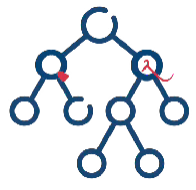
\includegraphics[height=0.9cm]{msca_logo.png}}%
  \end{center}
  \vspace{0.45cm}
  \begin{center}
    \begin{minipage}{0.1\textwidth}\centering
      \href{https://quantlet.com}{
\includegraphics[height=0.9cm]{ql_logo.png}}\end{minipage}%
    \begin{minipage}{0.78\textwidth}\centering
      {\Large\bfseries\usebeamercolor[fg]{title}\inserttitle}\par\vspace{0.25cm}
      {\large\usebeamercolor[fg]{title}\insertsubtitle}\end{minipage}%
    \begin{minipage}{0.1\textwidth}\centering
      \href{https://quantinar.com}{
\includegraphics[height=0.9cm]{qr_logo.png}}\end{minipage}
  \end{center}
  \vfill
  \hspace{0.4cm}{\bfseries\insertauthor}\par\vspace{0.12cm}
  \hspace{0.4cm}\begin{minipage}[t]{0.92\textwidth}\raggedright\footnotesize\insertinstitute\end{minipage}
  \par\vspace{0.4cm}}

% ---------------------------------------------------------------- lecture metadata
\newcommand{\emqashort}{}
\newcommand{\emqanb}{notebooks}
\newcommand{\emqarepo}{https://github.com/danpele/EMQA/tree/main}
% language-dependent labels (English default; \emqaromanian switches to Romanian, call it before \emqalecture)
\newcommand{\txtcourse}{Energy Markets Quantitative Analysis}
\newcommand{\txtlecture}{Lecture}
\newcommand{\txtoutline}{Outline}
\newcommand{\txtintuition}{In one sentence:}
\newcommand{\txtjob}{In practice:}
\newcommand{\txttry}{Experiment yourself:}
\newcommand{\txtwhere}{where}
\newcommand{\txtsim}{SIMULATED DATA (teaching illustration)}
\newcommand{\txtnbsuffix}{}
\newcommand{\txtinstitute}{Bucharest University of Economic Studies, Department of Statistics and Econometrics\\
    Romanian Academy, Institute for Economic Forecasting\\
    IDA Institute Digital Assets \textbullet\ AI4EFin \textbullet\ MSCA Digital Finance}
\newcommand{\emqaromanian}{%
  \renewcommand{\txtcourse}{Analiza cantitativă a piețelor de energie}%
  \renewcommand{\txtlecture}{Cursul}%
  \renewcommand{\txtoutline}{Cuprins}%
  \renewcommand{\txtintuition}{Pe scurt:}%
  \renewcommand{\txtjob}{În practică:}%
  \renewcommand{\txttry}{Exercițiu practic:}%
  \renewcommand{\txtwhere}{unde}%
  \renewcommand{\txtsim}{DATE SIMULATE (doar pentru ilustrare)}%
  \renewcommand{\txtnbsuffix}{\string_ro}%
  \renewcommand{\txtinstitute}{Academia de Studii Economice din București, Departamentul de Statistică și Econometrie\\
    Academia Română, Institutul de Prognoză Economică\\
    IDA Institute Digital Assets \textbullet\ AI4EFin \textbullet\ MSCA Digital Finance}}
\newcommand{\emqalecture}[2]{%
  \renewcommand{\emqashort}{\txtlecture\ #1}%
  \renewcommand{\emqanb}{notebooks/L#1\string_notebook\txtnbsuffix.ipynb}%
  \title[EMQA]{\txtcourse}%
  \subtitle{\txtlecture\ #1: #2}%
  \author{Prof.\ dr.\ Daniel Traian PELE}%
  \institute{\txtinstitute}%
  \date{}}

% ---------------------------------------------------------------- teaching blocks (MBA clarity rule)
% \intuition{one plain sentence}  ->  formula with every symbol defined  ->  real-data example  ->  \manager{one line}
\newcommand{\intuition}[1]{\begin{itemize}\item {\color{MainBlue}\textbf{\txtintuition}}~#1\end{itemize}\vspace{0.6mm}}
\newcommand{\manager}[1]{\colorbox{Forest!10}{\parbox{\dimexpr\linewidth-2\fboxsep\relax}{\footnotesize
  \begin{itemize}\setlength{\itemsep}{0pt}\item \textbf{\color{Forest}\txtjob}~#1\end{itemize}}}}
% Experiment yourself: pointer to the matching notebook section
\newcommand{\tryit}[1]{{\scriptsize\href{\emqarepo/\emqanb}{%
  \raisebox{-0.15em}{
\includegraphics[height=0.85em]{ql_logo.png}}\,\textbf{\txttry}~\color{MainBlue}#1}}}
% bottom row: manager line (left) + experiment pointer (right), pinned to the bottom of the frame
\newcommand{\bottomrow}[2]{\par\vfill\noindent\begin{minipage}[b]{0.72\linewidth}#1\end{minipage}\hfill
  \begin{minipage}[b]{0.26\linewidth}\raggedleft #2\end{minipage}\par\vspace{0.5mm}}
\newcommand{\where}[1]{{\footnotesize\textbf{\txtwhere}~#1\par}}

% ---------------------------------------------------------------- helpers
% chart source line under a figure: \chartsource{Source ...; period ...}
\newcommand{\chartsource}[1]{\par\vspace{1pt}{\scriptsize\color{FooterGray}#1\par}}
% link to code: \quantlet{label}{path inside the repo}
\newcommand{\quantlet}[2]{\par\vspace{1pt}\hfill\href{\emqarepo/#2}{%
  \raisebox{-0.15em}{
\includegraphics[height=0.75em]{ql_logo.png}}\textcolor{MainBlue}{\scriptsize\ #1}}}
\newcommand{\simlabel}{\colorbox{Crimson!12}{\scriptsize\bfseries\color{Crimson}\txtsim}}
\newcommand{\E}{\mathbb{E}}
\newcommand{\Var}{\operatorname{Var}}
\newcommand{\Cov}{\operatorname{Cov}}
\newcommand{\Corr}{\operatorname{Corr}}
\newcommand{\asinh}{\operatorname{asinh}}
\newcommand{\iid}{\overset{\text{i.i.d.}}{\sim}}
\newcommand{\EUR}{EUR}

%   \emqalecture{k}{Lecture title}
% Logos live in lectures/common/logos/, charts in lectures/Lk/charts/.
% Do NOT add \hfuzz / \vfuzz / \hbadness here: overfull boxes must be fixed, not hidden.
% =============================================================================

\usetheme{default}
\setbeamersize{text margin left=7mm, text margin right=7mm}

% ---------------------------------------------------------------- packages
\usepackage[utf8]{inputenc}
\usepackage[T1]{fontenc}
\usepackage{lmodern}
\usepackage{amsmath, amssymb}
\usepackage{mathtools}
\usepackage{bm}
\usepackage{tikz}
\usetikzlibrary{arrows.meta, positioning, calc, shapes.misc}
\usepackage{booktabs}
\usepackage{array}
\usepackage{graphicx}
\usepackage{colortbl}
\usepackage{xcolor}
\usepackage{multicol}
\hypersetup{colorlinks=true, linkcolor=MainBlue, urlcolor=MainBlue, citecolor=MainBlue}
\graphicspath{{../common/logos/}}   % charts are included with their language folder: charts/en/, charts/ro/

% ---------------------------------------------------------------- colours
\definecolor{MainBlue}{RGB}{26, 58, 110}
\definecolor{IDAred}{RGB}{205, 0, 0}
\definecolor{DarkGray}{RGB}{51, 51, 51}
\definecolor{FooterGray}{RGB}{100, 100, 100}
\definecolor{BlockGray}{RGB}{236, 238, 242}
\definecolor{KeynoteGray}{RGB}{218, 218, 218}
\definecolor{Crimson}{RGB}{190, 40, 50}
\definecolor{Forest}{RGB}{30, 110, 50}
\definecolor{Bitter}{RGB}{214, 150, 20}
% chart palette (same hex values as lectures/common/emqa_plot.py)
\definecolor{SerRO}{HTML}{2A78D6}
\definecolor{SerDE}{HTML}{EB6834}
\definecolor{SerHU}{HTML}{1BAF7A}
\definecolor{SerBG}{HTML}{EDA100}

\setbeamertemplate{background}{%
  \begin{tikzpicture}[remember picture, overlay]
    \shade[shading=axis, shading angle=315, top color=white, bottom color=KeynoteGray]
      (current page.south west) rectangle (current page.north east);
  \end{tikzpicture}}
\setbeamercolor{background canvas}{bg=}
\setbeamercolor{structure}{fg=MainBlue}
\setbeamercolor{normal text}{fg=DarkGray}
\setbeamercolor{title}{fg=IDAred}
\setbeamercolor{frametitle}{fg=IDAred, bg=}
\setbeamercolor{block title}{bg=MainBlue, fg=white}
\setbeamercolor{block body}{bg=BlockGray, fg=DarkGray}
\setbeamercolor{block title alerted}{bg=Crimson, fg=white}
\setbeamercolor{block body alerted}{bg=Crimson!7, fg=DarkGray}
\setbeamercolor{block title example}{bg=Forest, fg=white}
\setbeamercolor{block body example}{bg=Forest!7, fg=DarkGray}
\setbeamercolor{item}{fg=MainBlue}
\setbeamerfont{frametitle}{size=\large, series=\bfseries}
\setbeamerfont{block title}{size=\small, series=\bfseries}
\setbeamertemplate{blocks}[rounded][shadow=false]
\setbeamertemplate{itemize item}{\color{MainBlue}$\boxdot$}
\setbeamertemplate{itemize subitem}{\color{MainBlue}\scriptsize$\blacktriangleright$}
% compact two-level lists: level 1 = main point, level 2 = details (no text outside bullets)
\setbeamerfont{itemize/enumerate subbody}{size=\footnotesize}
\setlength{\leftmargini}{1.1em}
\setlength{\leftmarginii}{1.1em}
\setbeamertemplate{itemize/enumerate body begin}{\setlength{\topsep}{0pt}\setlength{\partopsep}{0pt}\setlength{\parskip}{0pt}}
\setbeamertemplate{itemize/enumerate subbody begin}{\setlength{\topsep}{0pt}\setlength{\partopsep}{0pt}\setlength{\itemsep}{0pt}\vspace{-0.4ex}}

\setbeamertemplate{enumerate item}{\color{MainBlue}\insertenumlabel.}
\setlength{\leftmargini}{1.3em}
\setlength{\leftmarginii}{1.2em}
\setbeamertemplate{navigation symbols}{}
\setbeamertemplate{section in toc}{\color{MainBlue}$\blacktriangleright$~\inserttocsection}
\setbeamertemplate{caption}{\raggedright\insertcaption\par}
% frame subtitle = precise citation line under the claim title (Weron style)
\setbeamerfont{framesubtitle}{size=\footnotesize}
\setbeamercolor{framesubtitle}{fg=FooterGray}
% outline that reappears at every section with the current section highlighted
\setbeamertemplate{section in toc shaded}[default][35]
\setbeamertemplate{subsection in toc shaded}[default][35]
\setbeamertemplate{subsection in toc}{\leavevmode\leftskip=2.2em\color{DarkGray}\small\inserttocsubsection\par}
\AtBeginSection[]{{\begin{frame}{\txtoutline}\vspace{2mm}\small
  \tableofcontents[currentsection,hideothersubsections]\end{frame}}}

% ---------------------------------------------------------------- head and foot
\setbeamertemplate{headline}{%
  \vskip10pt%
  \hbox to \paperwidth{\hskip0.5cm%
    {\small\color{FooterGray}\renewcommand{\hyperlink}[2]{##2}\insertsectionhead}%
    \hfill\textcolor{FooterGray}{\small\insertframenumber}\hskip0.5cm}%
  \vskip4pt{\color{FooterGray}\hrule height 0.4pt}}
% footer as in the other courses (MFM, SFM): course name on the left, small sparkline on the right
\setbeamertemplate{footline}{%
  {\color{FooterGray}\hrule height 0.4pt}\vskip4pt%
  \hbox to \paperwidth{\hskip0.5cm%
    \textcolor{FooterGray}{\small\txtcourse}%
    \hfill\raisebox{-0.1em}{\begin{tikzpicture}[x=0.08em, y=0.08em, line width=0.4pt]
      \draw[FooterGray] (0,3) -- (1,4) -- (2,3.5) -- (3,5) -- (4,4) -- (5,6) -- (6,5.5) -- (7,4) -- (8,5) -- (9,7) -- (10,6) -- (11,5) -- (12,6.5) -- (13,8) -- (14,7) -- (15,6) -- (16,7.5) -- (17,9) -- (18,8) -- (19,7) -- (20,8.5) -- (21,10) -- (22,9) -- (23,8) -- (24,9.5);
    \end{tikzpicture}}\hskip0.5cm}%
  \vskip6pt}

% ---------------------------------------------------------------- title page
\defbeamertemplate*{title page}{emqa}[1][]{%
  \vspace{0.15cm}
  \begin{center}
    \href{https://www.ase.ro}{
\includegraphics[height=0.9cm]{ase_logo.png}}\hspace{0.3cm}%
    \href{https://ipe.ro/new}{
\includegraphics[height=0.9cm]{acad_logo.png}}\hspace{0.3cm}%
    \href{https://theida.net}{
\includegraphics[height=0.9cm]{ida_logo.png}}\hspace{0.3cm}%
    \href{https://blockchain-research-center.com}{
\includegraphics[height=0.9cm]{brc_logo.png}}\hspace{0.3cm}%
    \href{https://www.ai4efin.ase.ro}{
\includegraphics[height=0.9cm]{ai4efin_logo.png}}\hspace{0.3cm}%
    \href{https://www.digital-finance-msca.com}{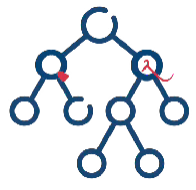
\includegraphics[height=0.9cm]{msca_logo.png}}%
  \end{center}
  \vspace{0.45cm}
  \begin{center}
    \begin{minipage}{0.1\textwidth}\centering
      \href{https://quantlet.com}{
\includegraphics[height=0.9cm]{ql_logo.png}}\end{minipage}%
    \begin{minipage}{0.78\textwidth}\centering
      {\Large\bfseries\usebeamercolor[fg]{title}\inserttitle}\par\vspace{0.25cm}
      {\large\usebeamercolor[fg]{title}\insertsubtitle}\end{minipage}%
    \begin{minipage}{0.1\textwidth}\centering
      \href{https://quantinar.com}{
\includegraphics[height=0.9cm]{qr_logo.png}}\end{minipage}
  \end{center}
  \vfill
  \hspace{0.4cm}{\bfseries\insertauthor}\par\vspace{0.12cm}
  \hspace{0.4cm}\begin{minipage}[t]{0.92\textwidth}\raggedright\footnotesize\insertinstitute\end{minipage}
  \par\vspace{0.4cm}}

% ---------------------------------------------------------------- lecture metadata
\newcommand{\emqashort}{}
\newcommand{\emqanb}{notebooks}
\newcommand{\emqarepo}{https://github.com/danpele/EMQA/tree/main}
% language-dependent labels (English default; \emqaromanian switches to Romanian, call it before \emqalecture)
\newcommand{\txtcourse}{Energy Markets Quantitative Analysis}
\newcommand{\txtlecture}{Lecture}
\newcommand{\txtoutline}{Outline}
\newcommand{\txtintuition}{In one sentence:}
\newcommand{\txtjob}{In practice:}
\newcommand{\txttry}{Experiment yourself:}
\newcommand{\txtwhere}{where}
\newcommand{\txtsim}{SIMULATED DATA (teaching illustration)}
\newcommand{\txtnbsuffix}{}
\newcommand{\txtinstitute}{Bucharest University of Economic Studies, Department of Statistics and Econometrics\\
    Romanian Academy, Institute for Economic Forecasting\\
    IDA Institute Digital Assets \textbullet\ AI4EFin \textbullet\ MSCA Digital Finance}
\newcommand{\emqaromanian}{%
  \renewcommand{\txtcourse}{Analiza cantitativă a piețelor de energie}%
  \renewcommand{\txtlecture}{Cursul}%
  \renewcommand{\txtoutline}{Cuprins}%
  \renewcommand{\txtintuition}{Pe scurt:}%
  \renewcommand{\txtjob}{În practică:}%
  \renewcommand{\txttry}{Exercițiu practic:}%
  \renewcommand{\txtwhere}{unde}%
  \renewcommand{\txtsim}{DATE SIMULATE (doar pentru ilustrare)}%
  \renewcommand{\txtnbsuffix}{\string_ro}%
  \renewcommand{\txtinstitute}{Academia de Studii Economice din București, Departamentul de Statistică și Econometrie\\
    Academia Română, Institutul de Prognoză Economică\\
    IDA Institute Digital Assets \textbullet\ AI4EFin \textbullet\ MSCA Digital Finance}}
\newcommand{\emqalecture}[2]{%
  \renewcommand{\emqashort}{\txtlecture\ #1}%
  \renewcommand{\emqanb}{notebooks/L#1\string_notebook\txtnbsuffix.ipynb}%
  \title[EMQA]{\txtcourse}%
  \subtitle{\txtlecture\ #1: #2}%
  \author{Prof.\ dr.\ Daniel Traian PELE}%
  \institute{\txtinstitute}%
  \date{}}

% ---------------------------------------------------------------- teaching blocks (MBA clarity rule)
% \intuition{one plain sentence}  ->  formula with every symbol defined  ->  real-data example  ->  \manager{one line}
\newcommand{\intuition}[1]{\begin{itemize}\item {\color{MainBlue}\textbf{\txtintuition}}~#1\end{itemize}\vspace{0.6mm}}
\newcommand{\manager}[1]{\colorbox{Forest!10}{\parbox{\dimexpr\linewidth-2\fboxsep\relax}{\footnotesize
  \begin{itemize}\setlength{\itemsep}{0pt}\item \textbf{\color{Forest}\txtjob}~#1\end{itemize}}}}
% Experiment yourself: pointer to the matching notebook section
\newcommand{\tryit}[1]{{\scriptsize\href{\emqarepo/\emqanb}{%
  \raisebox{-0.15em}{
\includegraphics[height=0.85em]{ql_logo.png}}\,\textbf{\txttry}~\color{MainBlue}#1}}}
% bottom row: manager line (left) + experiment pointer (right), pinned to the bottom of the frame
\newcommand{\bottomrow}[2]{\par\vfill\noindent\begin{minipage}[b]{0.72\linewidth}#1\end{minipage}\hfill
  \begin{minipage}[b]{0.26\linewidth}\raggedleft #2\end{minipage}\par\vspace{0.5mm}}
\newcommand{\where}[1]{{\footnotesize\textbf{\txtwhere}~#1\par}}

% ---------------------------------------------------------------- helpers
% chart source line under a figure: \chartsource{Source ...; period ...}
\newcommand{\chartsource}[1]{\par\vspace{1pt}{\scriptsize\color{FooterGray}#1\par}}
% link to code: \quantlet{label}{path inside the repo}
\newcommand{\quantlet}[2]{\par\vspace{1pt}\hfill\href{\emqarepo/#2}{%
  \raisebox{-0.15em}{
\includegraphics[height=0.75em]{ql_logo.png}}\textcolor{MainBlue}{\scriptsize\ #1}}}
\newcommand{\simlabel}{\colorbox{Crimson!12}{\scriptsize\bfseries\color{Crimson}\txtsim}}
\newcommand{\E}{\mathbb{E}}
\newcommand{\Var}{\operatorname{Var}}
\newcommand{\Cov}{\operatorname{Cov}}
\newcommand{\Corr}{\operatorname{Corr}}
\newcommand{\asinh}{\operatorname{asinh}}
\newcommand{\iid}{\overset{\text{i.i.d.}}{\sim}}
\newcommand{\EUR}{EUR}

%   \emqalecture{k}{Lecture title}
% Logos live in lectures/common/logos/, charts in lectures/Lk/charts/.
% Do NOT add \hfuzz / \vfuzz / \hbadness here: overfull boxes must be fixed, not hidden.
% =============================================================================

\usetheme{default}
\setbeamersize{text margin left=7mm, text margin right=7mm}

% ---------------------------------------------------------------- packages
\usepackage[utf8]{inputenc}
\usepackage[T1]{fontenc}
\usepackage{lmodern}
\usepackage{amsmath, amssymb}
\usepackage{mathtools}
\usepackage{bm}
\usepackage{tikz}
\usetikzlibrary{arrows.meta, positioning, calc, shapes.misc}
\usepackage{booktabs}
\usepackage{array}
\usepackage{graphicx}
\usepackage{colortbl}
\usepackage{xcolor}
\usepackage{multicol}
\hypersetup{colorlinks=true, linkcolor=MainBlue, urlcolor=MainBlue, citecolor=MainBlue}
\graphicspath{{../common/logos/}}   % charts are included with their language folder: charts/en/, charts/ro/

% ---------------------------------------------------------------- colours
\definecolor{MainBlue}{RGB}{26, 58, 110}
\definecolor{IDAred}{RGB}{205, 0, 0}
\definecolor{DarkGray}{RGB}{51, 51, 51}
\definecolor{FooterGray}{RGB}{100, 100, 100}
\definecolor{BlockGray}{RGB}{236, 238, 242}
\definecolor{KeynoteGray}{RGB}{218, 218, 218}
\definecolor{Crimson}{RGB}{190, 40, 50}
\definecolor{Forest}{RGB}{30, 110, 50}
\definecolor{Bitter}{RGB}{214, 150, 20}
% chart palette (same hex values as lectures/common/emqa_plot.py)
\definecolor{SerRO}{HTML}{2A78D6}
\definecolor{SerDE}{HTML}{EB6834}
\definecolor{SerHU}{HTML}{1BAF7A}
\definecolor{SerBG}{HTML}{EDA100}

\setbeamertemplate{background}{%
  \begin{tikzpicture}[remember picture, overlay]
    \shade[shading=axis, shading angle=315, top color=white, bottom color=KeynoteGray]
      (current page.south west) rectangle (current page.north east);
  \end{tikzpicture}}
\setbeamercolor{background canvas}{bg=}
\setbeamercolor{structure}{fg=MainBlue}
\setbeamercolor{normal text}{fg=DarkGray}
\setbeamercolor{title}{fg=IDAred}
\setbeamercolor{frametitle}{fg=IDAred, bg=}
\setbeamercolor{block title}{bg=MainBlue, fg=white}
\setbeamercolor{block body}{bg=BlockGray, fg=DarkGray}
\setbeamercolor{block title alerted}{bg=Crimson, fg=white}
\setbeamercolor{block body alerted}{bg=Crimson!7, fg=DarkGray}
\setbeamercolor{block title example}{bg=Forest, fg=white}
\setbeamercolor{block body example}{bg=Forest!7, fg=DarkGray}
\setbeamercolor{item}{fg=MainBlue}
\setbeamerfont{frametitle}{size=\large, series=\bfseries}
\setbeamerfont{block title}{size=\small, series=\bfseries}
\setbeamertemplate{blocks}[rounded][shadow=false]
\setbeamertemplate{itemize item}{\color{MainBlue}$\boxdot$}
\setbeamertemplate{itemize subitem}{\color{MainBlue}\scriptsize$\blacktriangleright$}
% compact two-level lists: level 1 = main point, level 2 = details (no text outside bullets)
\setbeamerfont{itemize/enumerate subbody}{size=\footnotesize}
\setlength{\leftmargini}{1.1em}
\setlength{\leftmarginii}{1.1em}
\setbeamertemplate{itemize/enumerate body begin}{\setlength{\topsep}{0pt}\setlength{\partopsep}{0pt}\setlength{\parskip}{0pt}}
\setbeamertemplate{itemize/enumerate subbody begin}{\setlength{\topsep}{0pt}\setlength{\partopsep}{0pt}\setlength{\itemsep}{0pt}\vspace{-0.4ex}}

\setbeamertemplate{enumerate item}{\color{MainBlue}\insertenumlabel.}
\setlength{\leftmargini}{1.3em}
\setlength{\leftmarginii}{1.2em}
\setbeamertemplate{navigation symbols}{}
\setbeamertemplate{section in toc}{\color{MainBlue}$\blacktriangleright$~\inserttocsection}
\setbeamertemplate{caption}{\raggedright\insertcaption\par}
% frame subtitle = precise citation line under the claim title (Weron style)
\setbeamerfont{framesubtitle}{size=\footnotesize}
\setbeamercolor{framesubtitle}{fg=FooterGray}
% outline that reappears at every section with the current section highlighted
\setbeamertemplate{section in toc shaded}[default][35]
\setbeamertemplate{subsection in toc shaded}[default][35]
\setbeamertemplate{subsection in toc}{\leavevmode\leftskip=2.2em\color{DarkGray}\small\inserttocsubsection\par}
\AtBeginSection[]{{\begin{frame}{\txtoutline}\vspace{2mm}\small
  \tableofcontents[currentsection,hideothersubsections]\end{frame}}}

% ---------------------------------------------------------------- head and foot
\setbeamertemplate{headline}{%
  \vskip10pt%
  \hbox to \paperwidth{\hskip0.5cm%
    {\small\color{FooterGray}\renewcommand{\hyperlink}[2]{##2}\insertsectionhead}%
    \hfill\textcolor{FooterGray}{\small\insertframenumber}\hskip0.5cm}%
  \vskip4pt{\color{FooterGray}\hrule height 0.4pt}}
% footer as in the other courses (MFM, SFM): course name on the left, small sparkline on the right
\setbeamertemplate{footline}{%
  {\color{FooterGray}\hrule height 0.4pt}\vskip4pt%
  \hbox to \paperwidth{\hskip0.5cm%
    \textcolor{FooterGray}{\small\txtcourse}%
    \hfill\raisebox{-0.1em}{\begin{tikzpicture}[x=0.08em, y=0.08em, line width=0.4pt]
      \draw[FooterGray] (0,3) -- (1,4) -- (2,3.5) -- (3,5) -- (4,4) -- (5,6) -- (6,5.5) -- (7,4) -- (8,5) -- (9,7) -- (10,6) -- (11,5) -- (12,6.5) -- (13,8) -- (14,7) -- (15,6) -- (16,7.5) -- (17,9) -- (18,8) -- (19,7) -- (20,8.5) -- (21,10) -- (22,9) -- (23,8) -- (24,9.5);
    \end{tikzpicture}}\hskip0.5cm}%
  \vskip6pt}

% ---------------------------------------------------------------- title page
\defbeamertemplate*{title page}{emqa}[1][]{%
  \vspace{0.15cm}
  \begin{center}
    \href{https://www.ase.ro}{
\includegraphics[height=0.9cm]{ase_logo.png}}\hspace{0.3cm}%
    \href{https://ipe.ro/new}{
\includegraphics[height=0.9cm]{acad_logo.png}}\hspace{0.3cm}%
    \href{https://theida.net}{
\includegraphics[height=0.9cm]{ida_logo.png}}\hspace{0.3cm}%
    \href{https://blockchain-research-center.com}{
\includegraphics[height=0.9cm]{brc_logo.png}}\hspace{0.3cm}%
    \href{https://www.ai4efin.ase.ro}{
\includegraphics[height=0.9cm]{ai4efin_logo.png}}\hspace{0.3cm}%
    \href{https://www.digital-finance-msca.com}{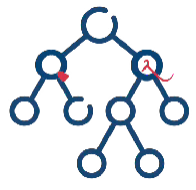
\includegraphics[height=0.9cm]{msca_logo.png}}%
  \end{center}
  \vspace{0.45cm}
  \begin{center}
    \begin{minipage}{0.1\textwidth}\centering
      \href{https://quantlet.com}{
\includegraphics[height=0.9cm]{ql_logo.png}}\end{minipage}%
    \begin{minipage}{0.78\textwidth}\centering
      {\Large\bfseries\usebeamercolor[fg]{title}\inserttitle}\par\vspace{0.25cm}
      {\large\usebeamercolor[fg]{title}\insertsubtitle}\end{minipage}%
    \begin{minipage}{0.1\textwidth}\centering
      \href{https://quantinar.com}{
\includegraphics[height=0.9cm]{qr_logo.png}}\end{minipage}
  \end{center}
  \vfill
  \hspace{0.4cm}{\bfseries\insertauthor}\par\vspace{0.12cm}
  \hspace{0.4cm}\begin{minipage}[t]{0.92\textwidth}\raggedright\footnotesize\insertinstitute\end{minipage}
  \par\vspace{0.4cm}}

% ---------------------------------------------------------------- lecture metadata
\newcommand{\emqashort}{}
\newcommand{\emqanb}{notebooks}
\newcommand{\emqarepo}{https://github.com/danpele/EMQA/tree/main}
% language-dependent labels (English default; \emqaromanian switches to Romanian, call it before \emqalecture)
\newcommand{\txtcourse}{Energy Markets Quantitative Analysis}
\newcommand{\txtlecture}{Lecture}
\newcommand{\txtoutline}{Outline}
\newcommand{\txtintuition}{In one sentence:}
\newcommand{\txtjob}{In practice:}
\newcommand{\txttry}{Experiment yourself:}
\newcommand{\txtwhere}{where}
\newcommand{\txtsim}{SIMULATED DATA (teaching illustration)}
\newcommand{\txtnbsuffix}{}
\newcommand{\txtinstitute}{Bucharest University of Economic Studies, Department of Statistics and Econometrics\\
    Romanian Academy, Institute for Economic Forecasting\\
    IDA Institute Digital Assets \textbullet\ AI4EFin \textbullet\ MSCA Digital Finance}
\newcommand{\emqaromanian}{%
  \renewcommand{\txtcourse}{Analiza cantitativă a piețelor de energie}%
  \renewcommand{\txtlecture}{Cursul}%
  \renewcommand{\txtoutline}{Cuprins}%
  \renewcommand{\txtintuition}{Pe scurt:}%
  \renewcommand{\txtjob}{În practică:}%
  \renewcommand{\txttry}{Exercițiu practic:}%
  \renewcommand{\txtwhere}{unde}%
  \renewcommand{\txtsim}{DATE SIMULATE (doar pentru ilustrare)}%
  \renewcommand{\txtnbsuffix}{\string_ro}%
  \renewcommand{\txtinstitute}{Academia de Studii Economice din București, Departamentul de Statistică și Econometrie\\
    Academia Română, Institutul de Prognoză Economică\\
    IDA Institute Digital Assets \textbullet\ AI4EFin \textbullet\ MSCA Digital Finance}}
\newcommand{\emqalecture}[2]{%
  \renewcommand{\emqashort}{\txtlecture\ #1}%
  \renewcommand{\emqanb}{notebooks/L#1\string_notebook\txtnbsuffix.ipynb}%
  \title[EMQA]{\txtcourse}%
  \subtitle{\txtlecture\ #1: #2}%
  \author{Prof.\ dr.\ Daniel Traian PELE}%
  \institute{\txtinstitute}%
  \date{}}

% ---------------------------------------------------------------- teaching blocks (MBA clarity rule)
% \intuition{one plain sentence}  ->  formula with every symbol defined  ->  real-data example  ->  \manager{one line}
\newcommand{\intuition}[1]{\begin{itemize}\item {\color{MainBlue}\textbf{\txtintuition}}~#1\end{itemize}\vspace{0.6mm}}
\newcommand{\manager}[1]{\colorbox{Forest!10}{\parbox{\dimexpr\linewidth-2\fboxsep\relax}{\footnotesize
  \begin{itemize}\setlength{\itemsep}{0pt}\item \textbf{\color{Forest}\txtjob}~#1\end{itemize}}}}
% Experiment yourself: pointer to the matching notebook section
\newcommand{\tryit}[1]{{\scriptsize\href{\emqarepo/\emqanb}{%
  \raisebox{-0.15em}{
\includegraphics[height=0.85em]{ql_logo.png}}\,\textbf{\txttry}~\color{MainBlue}#1}}}
% bottom row: manager line (left) + experiment pointer (right), pinned to the bottom of the frame
\newcommand{\bottomrow}[2]{\par\vfill\noindent\begin{minipage}[b]{0.72\linewidth}#1\end{minipage}\hfill
  \begin{minipage}[b]{0.26\linewidth}\raggedleft #2\end{minipage}\par\vspace{0.5mm}}
\newcommand{\where}[1]{{\footnotesize\textbf{\txtwhere}~#1\par}}

% ---------------------------------------------------------------- helpers
% chart source line under a figure: \chartsource{Source ...; period ...}
\newcommand{\chartsource}[1]{\par\vspace{1pt}{\scriptsize\color{FooterGray}#1\par}}
% link to code: \quantlet{label}{path inside the repo}
\newcommand{\quantlet}[2]{\par\vspace{1pt}\hfill\href{\emqarepo/#2}{%
  \raisebox{-0.15em}{
\includegraphics[height=0.75em]{ql_logo.png}}\textcolor{MainBlue}{\scriptsize\ #1}}}
\newcommand{\simlabel}{\colorbox{Crimson!12}{\scriptsize\bfseries\color{Crimson}\txtsim}}
\newcommand{\E}{\mathbb{E}}
\newcommand{\Var}{\operatorname{Var}}
\newcommand{\Cov}{\operatorname{Cov}}
\newcommand{\Corr}{\operatorname{Corr}}
\newcommand{\asinh}{\operatorname{asinh}}
\newcommand{\iid}{\overset{\text{i.i.d.}}{\sim}}
\newcommand{\EUR}{EUR}

\emqalecture{7}{Machine Learning for Energy Markets}
\begin{document}
{\setbeamertemplate{headline}{}\setbeamertemplate{footline}{}
\begin{frame}\titlepage\end{frame}}
% END-FRONT-MATTER

\begin{frame}{Learning objectives}
\small
\begin{itemize}\setlength{\itemsep}{1pt}
  \item Set up an honest machine learning (ML) experiment: training, validation and test samples in time order, and only the information known at 12:00 Central European Time (CET) on the day before delivery.
  \item Build and tune a deep neural network (DNN) and gradient-boosted trees for the 24 day-ahead prices of Romania
    \begin{itemize}\setlength{\itemsep}{0pt}
      \item Try a pretrained foundation model.
    \end{itemize}
  \item Compare them with the benchmarks of Lecture 2 on the same test year, with the mean absolute error (MAE), the root mean squared error (RMSE), the relative MAE (rMAE) and the Diebold--Mariano (DM) test
    \begin{itemize}\setlength{\itemsep}{0pt}
      \item Combine machine learning with the statistical models.
    \end{itemize}
  \item Explain the forecasts, predict price spikes and negative prices, and recognise the pitfalls that make a model look better than it is.
\end{itemize}
\end{frame}

% BEGIN-ABBR

\begin{frame}{Abbreviations (1/2)}
\small
\vspace{-1mm}\begin{columns}[T,onlytextwidth]
\begin{column}{0.49\textwidth}{\scriptsize\renewcommand{\arraystretch}{0.96}\begin{tabular}{@{}>{\bfseries}l@{\ \ }p{0.76\linewidth}@{}}AI & artificial intelligence\\
ARIMA & autoregressive integrated moving average\\
ARX & autoregressive model with exogenous variables\\
AUC & area under the ROC curve\\
AW & averaging across calibration windows\\
AW-ARX & ARX averaged across calibration windows\\
AW-LEAR & LEAR averaged across calibration windows\\
CET & Central European Time\\
CPU & central processing unit (processor core)\\
DM & Diebold--Mariano test\\
DNN & deep neural network\\\end{tabular}}\end{column}
\begin{column}{0.49\textwidth}{\scriptsize\renewcommand{\arraystretch}{0.96}\begin{tabular}{@{}>{\bfseries}l@{\ \ }p{0.76\linewidth}@{}}DST & daylight saving time\\
ENTSO-E & European Network of Transmission System Operators for Electricity\\
ETC & exchange-traded commodity\\
EU & European Union\\
EUA & EU emission allowance (1 t CO$_2$)\\
EUR & euro\\
FWER & familywise error rate\\
GBM & gradient boosting machine (boosted trees)\\
GW & gigawatt\\
ISE & Fraunhofer Institute for Solar Energy Systems\\
LASSO & least absolute shrinkage and selection operator\\\end{tabular}}\end{column}
\end{columns}
\end{frame}

\begin{frame}{Abbreviations (2/2)}
\small
\vspace{-1mm}\begin{columns}[T,onlytextwidth]
\begin{column}{0.49\textwidth}{\scriptsize\renewcommand{\arraystretch}{0.96}\begin{tabular}{@{}>{\bfseries}l@{\ \ }p{0.76\linewidth}@{}}LEAR & LASSO-estimated autoregression\\
LLM & large language model\\
MAD & median absolute deviation\\
MAE & mean absolute error\\
ML & machine learning\\
MLP & multilayer perceptron (feed-forward neural network)\\
MW & megawatt\\
MWh & megawatt-hour\\
OPCOM & Romanian electricity and gas market operator\\
PZU & Piața pentru Ziua Următoare (day-ahead market)\\
RC & Reality Check (data-snooping test of White, 2000)\\\end{tabular}}\end{column}
\begin{column}{0.49\textwidth}{\scriptsize\renewcommand{\arraystretch}{0.96}\begin{tabular}{@{}>{\bfseries}l@{\ \ }p{0.76\linewidth}@{}}ReLU & rectified linear unit\\
RES & renewable energy sources (here: wind + solar)\\
rMAE & relative MAE (model MAE / naive MAE)\\
RMSE & root mean squared error\\
RO & Romania (bidding zone)\\
ROC & receiver operating characteristic\\
SHAP & SHapley Additive exPlanations\\
SMAPE & symmetric mean absolute percentage error\\
SPA & superior predictive ability (test of Hansen, 2005)\\
TSO & transmission system operator\\
XGBoost & eXtreme Gradient Boosting (library)\\\end{tabular}}\end{column}
\end{columns}
\end{frame}

% END-ABBR

\begin{frame}{Same data, same test year as Lecture 2, plus a validation year}
\footnotesize
{\scriptsize\renewcommand{\arraystretch}{1.0}\setlength{\tabcolsep}{4pt}
\begin{tabular}{@{}p{0.24\textwidth}p{0.70\textwidth}@{}}\toprule
Element & Choice in this lecture \\ \midrule
Target & hourly day-ahead price of Romania (RO), Piața pentru Ziua Următoare (PZU), run by the Romanian electricity and gas market operator (OPCOM) \\
Inputs (as in Lecture 2) & prices up to $d-1$; load, wind + solar, hydro, nuclear, net imports up to $d-2$, from the European Network of Transmission System Operators for Electricity (ENTSO-E); carbon: European Union (EU) emission allowance (EUA), via an exchange-traded commodity (ETC) \\
Training & from 8 Jan 2022; grows by one month at each refit \\
Validation year & 1 Nov 2024 -- 31 Oct 2025: used only to choose the settings of the models \\
Test year & 1 Nov 2025 -- 31 Oct 2026, 8\,760 hours, models refitted monthly \\
\bottomrule\end{tabular}}
\vspace{1mm}
\begin{itemize}\setlength{\itemsep}{1pt}
  \item \textbf{Data up to 31 Oct 2026}, downloaded 4 Nov 2026 from energy-charts.info (Fraunhofer ISE) and Yahoo Finance.
  \item \textbf{Benchmarks}: the forecasts of Lecture 2, read from its files
    \begin{itemize}\setlength{\itemsep}{0pt}
      \item Naive model; autoregressive model with exogenous variables (ARX); least absolute shrinkage and selection operator (LASSO)
      \item LASSO-estimated autoregression (LEAR); ARX averaged across calibration windows (AW-ARX), LEAR likewise (AW-LEAR); ensemble of 4 models
    \end{itemize}
\end{itemize}
\par\vfill\noindent{\scriptsize\color{FooterGray}}\hfill\tryit{notebook \S1}\par\vspace{0.5mm}
\end{frame}


\section{Machine learning, evaluated honestly}

\begin{frame}{Machine learning buys flexibility and pays for it with variance}
\footnotesize
\intuition{A flexible model can learn thresholds and interactions that LEAR misses, but it can also learn the noise of the training years.}
\begin{columns}[T,onlytextwidth]
\begin{column}{0.52\textwidth}
\[ \hat\theta=\arg\min_{\theta}\ \underbrace{\frac1n\sum_{i=1}^{n}\ell\big(Y_i,f_\theta(\mathbf x_i)\big)}_{\text{fit to the training days}}+\underbrace{\lambda\,\Omega(\theta)}_{\text{penalty}} \]{\footnotesize\begin{itemize}\setlength{\itemsep}{0pt}
  \item \textbf{\txtwhere}
    \begin{itemize}\setlength{\itemsep}{0pt}
      \item $f_\theta$ = the model with parameters $\theta$
      \item $\mathbf x_i$ = inputs known at gate closure
      \item $Y_i$ = price
      \item $\ell$ = loss, here the absolute error
      \item $\Omega$ = complexity, $\lambda$ = its weight.
    \end{itemize}
\end{itemize}\par}
\end{column}
\begin{column}{0.45\textwidth}
\begin{itemize}\setlength{\itemsep}{1pt}
  \item \textbf{How flexible are our models?}
    \begin{itemize}\setlength{\itemsep}{0pt}
      \item LEAR: at most 247 coefficients per hour
      \item Our DNN: 141\,336 parameters, for 1\,727 training days at the last refit
    \end{itemize}
  \item \textbf{Consequence}
    \begin{itemize}\setlength{\itemsep}{0pt}
      \item The training error says nothing about the future; only data the model has not seen can judge it
    \end{itemize}
\end{itemize}
\end{column}
\end{columns}
\par\vfill\manager{ask a vendor how many parameters the model has per day of history, and on which days its error was measured.}\par\vspace{0.5mm}
\par\vfill\noindent{\scriptsize\color{FooterGray}(Hastie, Tibshirani \& Friedman, 2009; Lago et al., 2021, APEN)}\hfill\tryit{notebook \S1}\par\vspace{0.5mm}
\end{frame}

\begin{frame}{Three samples in time order: training, validation, test}
\small
\begin{center}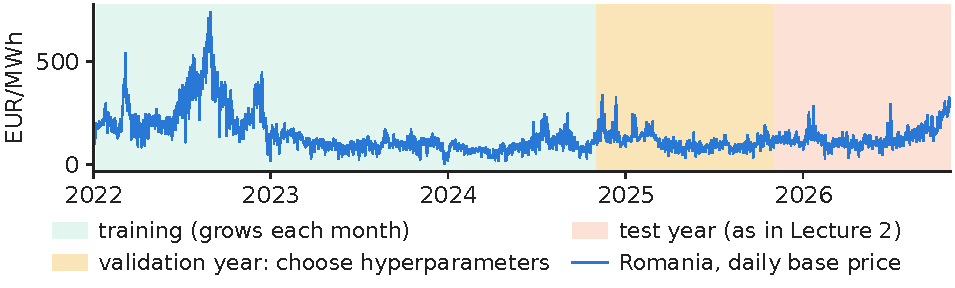
\includegraphics[width=\textwidth,height=0.477\textheight,keepaspectratio]{charts/en/split_ml.pdf}\end{center}\vspace{-3mm}
\chartsource{Source: energy-charts.info (Fraunhofer ISE): OPCOM prices. Data: daily base price, 2022-01-01 to 2026-10-31.}
\vspace{0.5mm}
\begin{itemize}\setlength{\itemsep}{0pt}
  \item \textbf{Validation year}: 25 settings per model compared, refitted every 3 months
    \begin{itemize}\setlength{\itemsep}{0pt}
      \item The setting with the lowest MAE is frozen before the test year starts
    \end{itemize}
  \item \textbf{Test year}: models refitted at the start of each month on all earlier days
    \begin{itemize}\setlength{\itemsep}{0pt}
      \item Never used to choose anything; the same year as in Lecture 2, so the errors are directly comparable
    \end{itemize}
\end{itemize}
\par\vfill\manager{treat the test year like a sealed envelope, opened once, after every choice is made.}\par\vspace{0.5mm}
\par\vfill\noindent{\scriptsize\color{FooterGray}(Bergmeir \& Benítez, 2012, Inf.\ Sci.; Lago et al., 2021, APEN)}\hfill\qlink{EMQA\_L7\_split\_ml}{Quantlets/L7/EMQA_L7_split_ml}\par\vspace{0.5mm}
\end{frame}

\begin{frame}{Hyperparameters are chosen by random search on the validation year}
\footnotesize
\intuition{Settings such as the number of neurons or of trees are not estimated by the model; we try several and keep the one that forecasts best on unseen days.}
\begin{columns}[T,onlytextwidth]
\begin{column}{0.55\textwidth}
\[ \gamma^{*}=\arg\min_{\gamma\in\{\gamma_0,\dots,\gamma_{24}\}}\ \frac{1}{24\,|\mathcal V|}\sum_{d\in\mathcal V}\sum_{h=0}^{23}\big|P_{d,h}-\hat P_{d,h}(\gamma)\big| \]{\footnotesize\begin{itemize}\setlength{\itemsep}{0pt}
  \item \textbf{\txtwhere}
    \begin{itemize}\setlength{\itemsep}{0pt}
      \item $\gamma$ = one setting (vector of hyperparameters)
      \item $\gamma_0$ = the setting of Lecture 2, the others drawn at random
      \item $\mathcal V$ = days of the validation year
      \item $\hat P_{d,h}(\gamma)$ = forecast with setting $\gamma$.
    \end{itemize}
\end{itemize}\par}
\end{column}
\begin{column}{0.42\textwidth}
\begin{itemize}\setlength{\itemsep}{1pt}
  \item \textbf{Why random, not a full grid}
    \begin{itemize}\setlength{\itemsep}{0pt}
      \item Only a few settings matter; random draws cover each of them better with the same budget
    \end{itemize}
  \item \textbf{Our budget}
    \begin{itemize}\setlength{\itemsep}{0pt}
      \item 24 random settings + the Lecture 2 setting, for each of the two models
      \item 7.3 minutes on one core of the central processing unit (CPU)
    \end{itemize}
\end{itemize}
\end{column}
\end{columns}
\par\vfill\manager{a modest, documented search is enough
    \begin{itemize}\setlength{\itemsep}{0pt}
      \item A search without a separate validation sample is not a search but a leak.
    \end{itemize}}\par\vspace{0.5mm}
\par\vfill\noindent{\scriptsize\color{FooterGray}(Bergstra \& Bengio, 2012, JMLR)}\hfill\tryit{notebook \S2}\par\vspace{0.5mm}
\end{frame}


\section{Deep neural networks}

\begin{frame}{A neural network stacks regressions, each followed by a bend}
\footnotesize
\intuition{Each neuron bends a linear combination of the inputs; the output layer gives the 24 prices of day $d$ at once.}
\begin{columns}[T,onlytextwidth]
\begin{column}{0.56\textwidth}
\[ \mathbf z=\phi\big(W_1\mathbf x_d+\mathbf b_1\big),\qquad \hat{\mathbf Y}_d=W_2\,\mathbf z+\mathbf b_2\in\mathbb R^{24} \]\[ \phi(u)=\max(0,u)\quad\text{or}\quad \phi(u)=\ln(1+e^{u}) \]{\footnotesize\begin{itemize}\setlength{\itemsep}{0pt}
  \item \textbf{\txtwhere}
    \begin{itemize}\setlength{\itemsep}{0pt}
      \item $\mathbf x_d$ = inputs of day $d$ (prices, load, wind + solar, fundamentals, weekday)
      \item $W_1,W_2$ = weights, $\mathbf b_1,\mathbf b_2$ = intercepts
      \item $\phi$ = rectified linear unit (ReLU) or its smooth version (softplus)
      \item $\hat{\mathbf Y}_d$ = asinh-scaled prices, as in Lecture 2.
    \end{itemize}
\end{itemize}\par}
\end{column}
\begin{column}{0.41\textwidth}
\begin{itemize}\setlength{\itemsep}{1pt}
  \item \textbf{Our network} (chosen on the validation year)
    \begin{itemize}\setlength{\itemsep}{0pt}
      \item 251 inputs, one hidden layer of 512 neurons, softplus, 24 outputs
      \item 141\,336 parameters; two-layer networks did worse on validation
    \end{itemize}
  \item \textbf{Better than in Lecture 2}
    \begin{itemize}\setlength{\itemsep}{0pt}
      \item The multilayer perceptron (MLP) of Lecture 2 had MAE 25.54; ours has 22.95 EUR/MWh
    \end{itemize}
\end{itemize}
\end{column}
\end{columns}
\par\vfill\manager{a network is a regression with many more coefficients: it needs the same data discipline, not less.}\par\vspace{0.5mm}
\par\vfill\noindent{\scriptsize\color{FooterGray}(Lago, Marcjasz, De Schutter \& Weron, 2021, APEN)}\hfill\tryit{notebook \S2}\par\vspace{0.5mm}
\end{frame}

\begin{frame}{Training: small steps against the error, stopped in time}
\footnotesize
\intuition{The weights move a little in the direction that lowers the error on a random batch of days; we stop when the error on later days stops falling.}
\begin{columns}[T,onlytextwidth]
\begin{column}{0.52\textwidth}
\[ \mathcal L(\theta)=\frac{1}{24\,|B|}\sum_{d\in B}\sum_{h=0}^{23}\big|Y_{d,h}-\hat Y_{d,h}(\theta)\big| \]\[ \theta\leftarrow\theta-\eta\,\widehat{\nabla\mathcal L} \]{\footnotesize\begin{itemize}\setlength{\itemsep}{0pt}
  \item \textbf{\txtwhere}
    \begin{itemize}\setlength{\itemsep}{0pt}
      \item $B$ = a mini-batch of 64 days
      \item $\eta$ = learning rate ($3\cdot10^{-4}$)
      \item $\widehat{\nabla\mathcal L}$ = gradient rescaled by the Adam method
      \item One epoch = one pass over all training days.
    \end{itemize}
\end{itemize}\par}
\end{column}
\begin{column}{0.45\textwidth}
\begin{itemize}\setlength{\itemsep}{1pt}
  \item \textbf{Early stopping}
    \begin{itemize}\setlength{\itemsep}{0pt}
      \item Train on the first 85\% of the training days, watch the error on the last 15\%
      \item Keep the best epoch, then refit on all days for that many epochs
    \end{itemize}
  \item \textbf{On our data}
    \begin{itemize}\setlength{\itemsep}{0pt}
      \item Epochs kept: median 56, from 23 to 92 (12 refits $\times$ 4 seeds)
      \item Dropout: during training each neuron is switched off at random with probability 0.1
    \end{itemize}
\end{itemize}
\end{column}
\end{columns}
\par\vfill\manager{the stopping rule uses only past days: it is part of the model, so it is checked like the rest.}\par\vspace{0.5mm}
\par\vfill\noindent{\scriptsize\color{FooterGray}(Kingma \& Ba, 2015, ICLR; Srivastava et al., 2014, JMLR)}\hfill\tryit{notebook \S2}\par\vspace{0.5mm}
\end{frame}

\begin{frame}{Early stopping: stop when the error on recent days stops falling}
\small
\begin{center}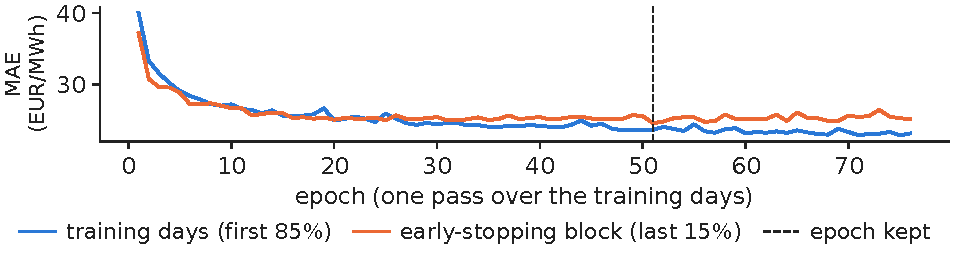
\includegraphics[width=\textwidth,height=0.500\textheight,keepaspectratio]{charts/en/learning_curve.pdf}\end{center}\vspace{-3mm}
\chartsource{Source: energy-charts.info (Fraunhofer ISE); Yahoo Finance (EUA). Data: chosen DNN, refit for 2026-10, seed 1.}
\vspace{0.5mm}
\begin{itemize}\setlength{\itemsep}{0pt}
  \item Refit for Oct 2026: the error on the last 15\% of days is lowest at epoch 51
    \begin{itemize}\setlength{\itemsep}{0pt}
      \item 24.50 EUR/MWh; training stops at epoch 76
    \end{itemize}
  \item After that point the network fits the past better and the recent days worse: it starts to memorise.
\end{itemize}
\par\vfill\manager{ask the vendor for this curve: without it, the network may simply have memorised the past.}\par\vspace{0.5mm}
\par\vfill\noindent{\scriptsize\color{FooterGray}(own computation; chosen DNN, seed 1)}\hfill\qlink{EMQA\_L7\_learning\_curve}{Quantlets/L7/EMQA_L7_learning_curve}\par\vspace{0.5mm}
\end{frame}

\begin{frame}{Random search cuts the validation error of both models}
\small
\begin{center}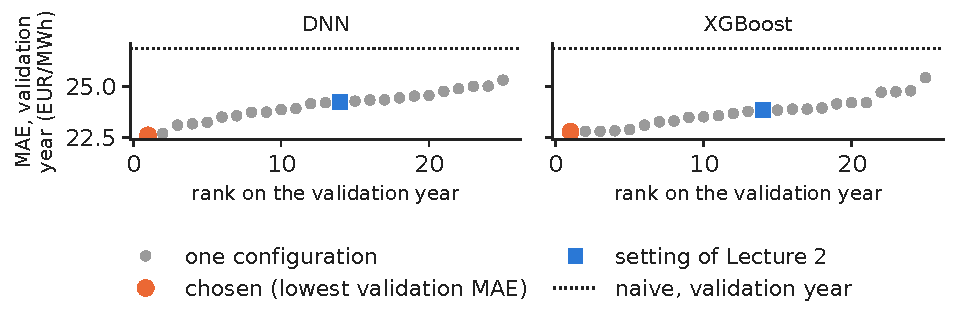
\includegraphics[width=\textwidth,height=0.502\textheight,keepaspectratio]{charts/en/search.pdf}\end{center}\vspace{-3mm}
\chartsource{Source: energy-charts.info (Fraunhofer ISE); Yahoo Finance (EUA). Data: validation year 2024-11-01 to 2025-10-31, quarterly refits.}
\vspace{0.5mm}
\begin{itemize}\setlength{\itemsep}{0pt}
  \item \textbf{DNN}: best setting 22.59 EUR/MWh; Lecture 2 setting 24.24, rank 14 of 25
    \begin{itemize}\setlength{\itemsep}{0pt}
      \item \textbf{eXtreme Gradient Boosting (XGBoost)}: 22.76 against 23.83 (rank 14)
    \end{itemize}
  \item All 25 settings of both models beat the naive model on the validation year (26.90 EUR/MWh).
\end{itemize}
\par\vfill\manager{budget one validation year for tuning any machine-learning model.}\par\vspace{0.5mm}
\par\vfill\noindent{\scriptsize\color{FooterGray}(own computation; validation year 1 Nov 2024 -- 31 Oct 2025)}\hfill\qlink{EMQA\_L7\_search}{Quantlets/L7/EMQA_L7_search}\par\vspace{0.5mm}
\end{frame}


\section{Gradient boosting and foundation models}

\begin{frame}{A regression tree cuts the inputs into boxes and predicts one price per box}
\footnotesize
\intuition{A tree asks yes/no questions; each final leaf holds one value, so thresholds and interactions come for free.}
\begin{columns}[T,onlytextwidth]
\begin{column}{0.60\textwidth}
\[ f(\mathbf x)=\textstyle\sum_{j=1}^{J}w_j\,\mathbb 1\{\mathbf x\in R_j\} \]\vspace{-1mm}\[ \text{Gain}=\frac{G_L^2}{H_L+\lambda}+\frac{G_R^2}{H_R+\lambda}-\frac{(G_L+G_R)^2}{H_L+H_R+\lambda}-\gamma \]{\footnotesize\begin{itemize}\setlength{\itemsep}{0pt}
  \item \textbf{\txtwhere}
    \begin{itemize}\setlength{\itemsep}{0pt}
      \item $R_j$ = leaf $j$, $w_j$ = its value
      \item $G$, $H$ = sums of the 1st and 2nd derivatives of the loss, left ($L$) and right ($R$)
      \item $\lambda$, $\gamma$ = penalties
      \item The split with the largest gain is kept.
    \end{itemize}
\end{itemize}\par}
\end{column}
\begin{column}{0.37\textwidth}
\begin{itemize}\setlength{\itemsep}{1pt}
  \item \textbf{On our data} (refit for Oct 2026)
    \begin{itemize}\setlength{\itemsep}{0pt}
      \item First question of the first tree: price of $d-1$, same hour, below 119.5 EUR/MWh?
      \item 233 leaves; the model adds up 1\,500 such trees
    \end{itemize}
\end{itemize}
\end{column}
\end{columns}
\par\vfill\manager{a tree speaks the language of a trading desk: above a level yesterday, a premium tonight.}\par\vspace{0.5mm}
\par\vfill\noindent{\scriptsize\color{FooterGray}(Chen \& Guestrin, 2016, KDD; Hastie et al., 2009)}\hfill\tryit{notebook \S3}\par\vspace{0.5mm}
\end{frame}

\begin{frame}{Gradient boosting: each new tree corrects the remaining errors}
\footnotesize
\intuition{Fit a small tree to what is still wrong, add it with a small weight, repeat a thousand times.}
\begin{columns}[T,onlytextwidth]
\begin{column}{0.57\textwidth}
\[ F_m(\mathbf x)=F_{m-1}(\mathbf x)+\eta\,f_m(\mathbf x),\qquad w_j^{*}=-\frac{G_j}{H_j+\lambda} \]\[ \min\ \textstyle\sum_{i}\ell\big(Y_i,F_M(\mathbf x_i)\big)+\sum_{m}\big(\gamma J_m+\tfrac{\lambda}{2}\sum_j w_{mj}^2\big) \]{\footnotesize\begin{itemize}\setlength{\itemsep}{0pt}
  \item \textbf{\txtwhere}
    \begin{itemize}\setlength{\itemsep}{0pt}
      \item $F_m$ = forecast after $m$ trees
      \item $f_m$ = tree $m$, with $J_m$ leaves
      \item $\eta$ = learning rate
      \item $w_j^{*}$ = optimal value of leaf $j$ (Appendix B)
      \item $\ell$ = absolute error.
    \end{itemize}
\end{itemize}\par}
\end{column}
\begin{column}{0.40\textwidth}
\begin{itemize}\setlength{\itemsep}{1pt}
  \item \textbf{Chosen on the validation year}
    \begin{itemize}\setlength{\itemsep}{0pt}
      \item 1\,500 trees of depth 8, $\eta$ = 0.02, each tree on a fraction 0.8 of the rows
    \end{itemize}
  \item \textbf{Test year}
    \begin{itemize}\setlength{\itemsep}{0pt}
      \item MAE 23.26 EUR/MWh; untuned gradient boosting machine (GBM) of Lecture 2: 24.05 (DM $p<0.001$)
      \item AW-LEAR (22.53) is still more accurate (DM $p$ = 0.016)
    \end{itemize}
\end{itemize}
\end{column}
\end{columns}
\par\vfill\manager{tuning matters more than the software: the same kind of trees gained almost one euro per MWh from good settings.}\par\vspace{0.5mm}
\par\vfill\noindent{\scriptsize\color{FooterGray}(Friedman, 2001, Ann.\ Stat.; Chen \& Guestrin, 2016, KDD)}\hfill\tryit{notebook \S3}\par\vspace{0.5mm}
\end{frame}

\begin{frame}{Foundation models forecast Romanian prices with no training at all}
\footnotesize
\intuition{Chronos models were trained by Amazon on large collections of time series; we give them only the recent prices and ask for the next 24 hours (zero-shot).}
\begin{columns}[T,onlytextwidth]
\begin{column}{0.52\textwidth}
\[ \big(\hat q^{\tau}_{d,h}\big)_{h=0,\dots,23}^{\tau=0.1,\,0.5,\,0.9}=g\big(P_{t-2047},\dots,P_{t}\big) \]{\footnotesize\begin{itemize}\setlength{\itemsep}{0pt}
  \item \textbf{\txtwhere}
    \begin{itemize}\setlength{\itemsep}{0pt}
      \item $P_{t-2047},\dots,P_t$ = the last 2048 hourly prices, up to the end of $d-1$ (85 days)
      \item $g$ = the pretrained network, used as it is
      \item $\hat q^{\tau}$ = forecast quantiles
      \item The point forecast is the median $\hat q^{0.5}$.
    \end{itemize}
\end{itemize}\par}
\end{column}
\begin{column}{0.45\textwidth}
\begin{itemize}\setlength{\itemsep}{1pt}
  \item \textbf{Test year}, prices only, no fundamentals
    \begin{itemize}\setlength{\itemsep}{0pt}
      \item Chronos-2: MAE 20.82; Chronos-Bolt: 22.15; AW-LEAR: 22.53 EUR/MWh
      \item Chronos-2 more accurate than AW-LEAR: DM $p<0.001$; in all 24 hours
    \end{itemize}
  \item \textbf{Robustness}
    \begin{itemize}\setlength{\itemsep}{0pt}
      \item Validation year: Chronos-2 21.05, best tuned DNN 22.59
      \item Published in Oct 2025, before the test year
    \end{itemize}
\end{itemize}
\end{column}
\end{columns}
\par\vfill\manager{test a foundation model before building your own network: it is cheap, and here it was the most accurate single model.}\par\vspace{0.5mm}
\par\vfill\noindent{\scriptsize\color{FooterGray}(Ansari et al., 2024, TMLR; Ansari et al., 2025, arXiv)}\hfill\tryit{notebook \S4}\par\vspace{0.5mm}
\end{frame}

\begin{frame}{Chronos-2 beats AW-LEAR in every hour of the day}
\small
\begin{center}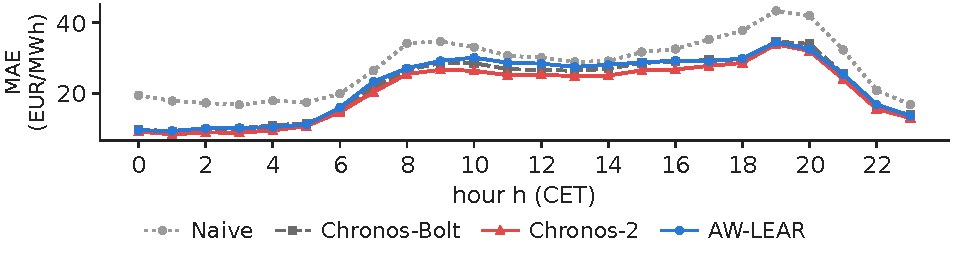
\includegraphics[width=\textwidth,height=0.437\textheight,keepaspectratio]{charts/en/foundation_hour.pdf}\end{center}\vspace{-3mm}
\chartsource{Source: energy-charts.info (Fraunhofer ISE): OPCOM prices. Data: test year 2025-11-01 to 2026-10-31; zero-shot, context = last 2048 hourly prices.}
\vspace{0.5mm}
\begin{itemize}\setlength{\itemsep}{0pt}
  \item Chronos-Bolt, smaller and older, is level with AW-LEAR (DM $p$ = 0.220).
  \item The 10\%--90\% band of Chronos-2 holds 76.5\% of the prices, not 80\%: too narrow.
\end{itemize}
\par\vfill\manager{use the median
    \begin{itemize}\setlength{\itemsep}{0pt}
      \item Recalibrate the bands (Lecture 2) before sizing risk with them.
    \end{itemize}}\par\vspace{0.5mm}
\par\vfill\noindent{\scriptsize\color{FooterGray}(own computation, test year 1 Nov 2025 -- 31 Oct 2026)}\hfill\qlink{EMQA\_L7\_foundation\_hour}{Quantlets/L7/EMQA_L7_foundation_hour}\par\vspace{0.5mm}
\end{frame}

\begin{frame}{AIDA 2026 keynote: deep networks beat LEAR, zero-shot models compete}
\footnotesize
\begin{columns}[T,onlytextwidth]
\begin{column}{0.50\textwidth}
\begin{itemize}\setlength{\itemsep}{1pt}
  \item \textbf{R.\ Weron, keynote} (4 June 2026, \href{https://github.com/danpele/EMQA/blob/main/resources/aida2026/weron_ml_electricity_price_forecasting.pdf}{slides})
    \begin{itemize}\setlength{\itemsep}{0pt}
      \item Model evolution: ARX, averaging across windows, LEAR, deep and interpretable networks
      \item Pretrained zero-shot models against LEAR and distributional DNN models, test 2021--2025
    \end{itemize}
  \item \textbf{Deep and interpretable networks}
    \begin{itemize}\setlength{\itemsep}{0pt}
      \item Open epftoolbox benchmark: the DNN had a lower rMAE than LEAR in all five markets (Lago et al., 2021)
      \item NBEATSx: trend, seasonality and exogenous blocks make the network readable (Olivares et al., 2023)
    \end{itemize}
\end{itemize}
\end{column}
\begin{column}{0.47\textwidth}
\begin{itemize}\setlength{\itemsep}{1pt}
  \item \textbf{Zero-shot results} (RMSE, as printed)
    \begin{itemize}\setlength{\itemsep}{0pt}
      \item 2022: LEAR + conformal prediction 45.71, Chronos 2 41.07, TabPFN 3.0 ts 34.39
      \item 2025: 20.38, 20.58, 17.66; a TabPFN version was the best in every year
    \end{itemize}
  \item \textbf{Link with our test year}
    \begin{itemize}\setlength{\itemsep}{0pt}
      \item Chronos-2, zero-shot, is our most accurate single model (MAE 20.82 vs 22.53 for AW-LEAR)
      \item Rankings move: TabPFN 2.0 had RMSE 68.85 in 2022, 17.52 in 2025
    \end{itemize}
\end{itemize}
\end{column}
\end{columns}
\par\vfill\manager{keep LEAR as the benchmark and test zero-shot models next to it, over several years.}\par\vspace{0.5mm}
\par\vfill\noindent{\scriptsize\color{FooterGray}(AIDA 2026 slides, Bucharest; papers: \href{https://doi.org/10.1016/j.apenergy.2021.116983}{Lago et al., 2021, APEN}; \href{https://doi.org/10.1016/j.ijforecast.2022.03.001}{Olivares et al., 2023, IJF})}\par\vspace{0.5mm}
\end{frame}

\begin{frame}{AIDA 2026: four generations of models on 27 European price series}
\footnotesize
\begin{columns}[T,onlytextwidth]
\begin{column}{0.52\textwidth}
\begin{itemize}\setlength{\itemsep}{1pt}
  \item \textbf{A.-V.\ Andrei et al., talk} (3 June 2026, \href{https://github.com/danpele/EMQA/blob/main/resources/aida2026/andrei_ai4efin_benchmarking.pdf}{slides})
    \begin{itemize}\setlength{\itemsep}{0pt}
      \item 11 models, four generations: econometric, e.g.\ autoregressive integrated moving average (ARIMA); deep learning; transformers; pretrained large language models (LLM): Chronos, TimesFM
    \end{itemize}
  \item \textbf{Data and walk-forward validation}
    \begin{itemize}\setlength{\itemsep}{0pt}
      \item Wholesale prices of 27 European Union (EU) countries, Ember (from ENTSO-E)
      \item 96 steps in, 96 out; training 2000 hours (83 days), test 500 hours (20 days)
      \item Symmetric mean absolute percentage error (SMAPE); score (100 $\times$ SMAPE + RMSE)/2
    \end{itemize}
\end{itemize}
\end{column}
\begin{column}{0.45\textwidth}
\begin{itemize}\setlength{\itemsep}{1pt}
  \item \textbf{Results} (rank among the 11 models)
    \begin{itemize}\setlength{\itemsep}{0pt}
      \item PatchTST (a transformer) is first or second in all 27 countries
      \item Romania: PatchTST 1, TimesFM 2, Chronos 8, ARIMA 9
      \item Germany: PatchTST 1, TimesFM 5, Chronos 10
      \item Gains are model-specific, not uniform across the 4th generation
    \end{itemize}
  \item \textbf{Link with this lecture}
    \begin{itemize}\setlength{\itemsep}{0pt}
      \item On Romanian prices, Chronos-2 (2025) is our best single model (MAE 20.82)
    \end{itemize}
\end{itemize}
\end{column}
\end{columns}
\par\vfill\manager{compare model generations with walk-forward validation on several markets before choosing one.}\par\vspace{0.5mm}
\par\vfill\noindent{\scriptsize\color{FooterGray}(AIDA 2026 slides, Bucharest; paper: \href{https://arxiv.org/abs/2411.03372}{Andrei et al., 2024, arXiv})}\par\vspace{0.5mm}
\end{frame}


\section{Honest comparison, combination and cost}

\begin{frame}{Scoreboard: Chronos-2 is the best single model}
\small
\begin{center}{\scriptsize\renewcommand{\arraystretch}{0.96}\setlength{\tabcolsep}{4pt}
\begin{tabular}{@{}lrrrrr@{}}\toprule
Model & MAE & RMSE & rMAE & vs AW-LEAR, \% & DM $p$ \\ \midrule
Naive & \cellcolor{Crimson!55}27.82 & \cellcolor{Crimson!55}44.54 & \cellcolor{Crimson!55}1.000 & \cellcolor{Crimson!55}\ensuremath{-}23.5 & -- \\
AW-ARX & \cellcolor{Forest!32}22.30 & \cellcolor{Forest!31}36.34 & \cellcolor{Forest!31}0.802 & \cellcolor{Forest!32}\ensuremath{+}1.0 & 0.203 \\
AW-LEAR & \cellcolor{Forest!28}22.53 & \cellcolor{Forest!31}36.35 & \cellcolor{Forest!28}0.810 & \cellcolor{Forest!28}\ensuremath{+}0.0 & -- \\
Ensemble of 4 (Lecture 2) & \cellcolor{Forest!34}22.13 & \cellcolor{Forest!38}35.76 & \cellcolor{Forest!34}0.795 & \cellcolor{Forest!34}\ensuremath{+}1.8 & 0.014 \\
GBM (Lecture 2) & \cellcolor{Forest!4}24.05 & \cellcolor{Forest!17}37.73 & \cellcolor{Forest!4}0.864 & \cellcolor{Forest!4}\ensuremath{-}6.7 & 1.000 \\
MLP (Lecture 2) & \cellcolor{Crimson!19}25.54 & \cellcolor{Crimson!8}40.05 & \cellcolor{Crimson!19}0.918 & \cellcolor{Crimson!19}\ensuremath{-}13.3 & 1.000 \\
XGBoost, tuned & \cellcolor{Forest!17}23.26 & \cellcolor{Forest!25}36.94 & \cellcolor{Forest!17}0.836 & \cellcolor{Forest!17}\ensuremath{-}3.2 & 0.984 \\
DNN, tuned & \cellcolor{Forest!21}22.95 & \cellcolor{Forest!31}36.42 & \cellcolor{Forest!21}0.825 & \cellcolor{Forest!22}\ensuremath{-}1.8 & 0.944 \\
Chronos-Bolt, zero-shot & \cellcolor{Forest!34}22.15 & \cellcolor{Forest!39}35.65 & \cellcolor{Forest!34}0.796 & \cellcolor{Forest!34}\ensuremath{+}1.7 & 0.220 \\
Chronos-2, zero-shot & \cellcolor{Forest!55}20.82 & \cellcolor{Forest!53}34.32 & \cellcolor{Forest!55}0.748 & \cellcolor{Forest!55}\ensuremath{+}7.6 & $<$0.001 \\
AW-LEAR + DNN + XGBoost & \cellcolor{Forest!37}21.97 & \cellcolor{Forest!41}35.42 & \cellcolor{Forest!37}0.790 & \cellcolor{Forest!37}\ensuremath{+}2.5 & 0.001 \\
AW-ARX + AW-LEAR + DNN + XGBoost & \cellcolor{Forest!41}21.69 & \cellcolor{Forest!43}35.25 & \cellcolor{Forest!41}0.779 & \cellcolor{Forest!42}\ensuremath{+}3.8 & $<$0.001 \\
AW-LEAR + Chronos-2 & \cellcolor{Forest!55}20.81 & \cellcolor{Forest!55}34.11 & \cellcolor{Forest!55}0.748 & \cellcolor{Forest!55}\ensuremath{+}7.6 & -- \\
Ensemble of 5 (with Chronos-2) & \cellcolor{Forest!50}21.12 & \cellcolor{Forest!51}34.50 & \cellcolor{Forest!50}0.759 & \cellcolor{Forest!50}\ensuremath{+}6.3 & $<$0.001 \\
\bottomrule\end{tabular}}\end{center}\vspace{-2mm}
\par\vspace{0.5mm}{\scriptsize \begin{itemize}\setlength{\itemsep}{0pt}
  \item Root mean squared error (RMSE); relative MAE (rMAE) = MAE / MAE of the naive model; green = better, per column.
  \item DM $p$: one-sided test that the model is more accurate than AW-LEAR (daily mean absolute error, Newey--West variance, as in Lecture 2).
\end{itemize}}
\par\vfill\noindent{\scriptsize\color{FooterGray}(own computation, test year 1 Nov 2025 -- 31 Oct 2026)}\hfill\tryit{notebook \S5}\par\vspace{0.5mm}
\end{frame}

\begin{frame}{DM tests: combinations with ML beat AW-LEAR significantly}
\small
\begin{center}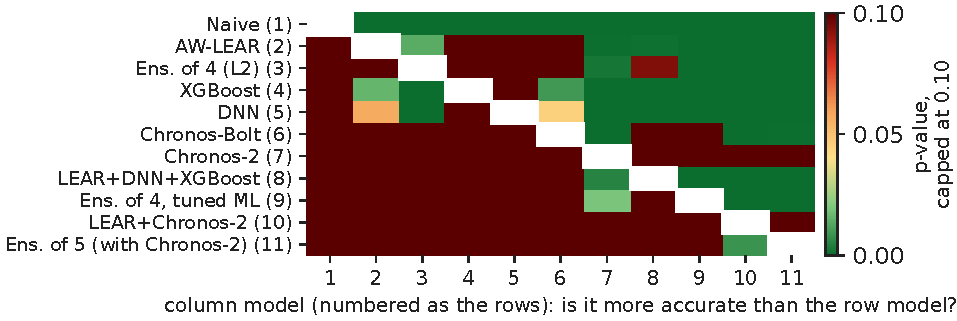
\includegraphics[width=\textwidth,height=0.502\textheight,keepaspectratio]{charts/en/dm_matrix.pdf}\end{center}\vspace{-3mm}
\chartsource{Source: energy-charts.info (Fraunhofer ISE); Yahoo Finance (EUA). Data: test year 2025-11-01 to 2026-10-31, 365 days; one-sided p-values.}
\vspace{0.5mm}
\begin{itemize}\setlength{\itemsep}{0pt}
  \item AW-LEAR + DNN + XGBoost beats AW-LEAR ($p$ = 0.001)
    \begin{itemize}\setlength{\itemsep}{0pt}
      \item Adding AW-ARX gives MAE 21.69, better than the Lecture 2 ensemble ($p<0.001$).
    \end{itemize}
  \item Adding AW-LEAR to Chronos-2 changes nothing ($p$ = 0.491): on the hard days the two models make similar errors.
\end{itemize}
\par\vfill\noindent{\scriptsize\color{FooterGray}(own computation; one-sided DM tests)}\hfill\qlink{EMQA\_L7\_dm\_matrix}{Quantlets/L7/EMQA_L7_dm_matrix}\par\vspace{0.5mm}
\end{frame}

\begin{frame}{Averaging works because the errors are not identical}
\small
\begin{center}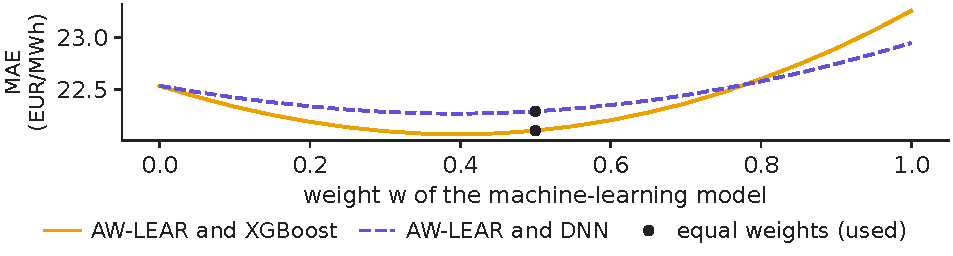
\includegraphics[width=\textwidth,height=0.416\textheight,keepaspectratio]{charts/en/combo_weight.pdf}\end{center}\vspace{-3mm}
\chartsource{Source: energy-charts.info (Fraunhofer ISE); Yahoo Finance (EUA). Data: test year 2025-11-01 to 2026-10-31; illustration, the weight is not chosen on the test year.}
\vspace{0.5mm}
\begin{itemize}\setlength{\itemsep}{0pt}
  \item $\Var\big(\tfrac{e_1+e_2}{2}\big)=\tfrac14(\sigma_1^2+\sigma_2^2+2\rho\sigma_1\sigma_2)$: with correlation $\rho<1$, the average errs less ($e$ = error, $\sigma$ = its standard deviation).
  \item Error correlation with AW-LEAR: 0.94 (DNN), 0.89 (XGBoost)
    \begin{itemize}\setlength{\itemsep}{0pt}
      \item Equal weights do almost as well as the best weight seen afterwards (0.40).
    \end{itemize}
\end{itemize}
\par\vfill\manager{average with equal weights before estimating clever weights.}\par\vspace{0.5mm}
\par\vfill\noindent{\scriptsize\color{FooterGray}(Bates \& Granger, 1969; own computation)}\hfill\qlink{EMQA\_L7\_combo\_weight}{Quantlets/L7/EMQA_L7_combo_weight}\par\vspace{0.5mm}
\end{frame}

\begin{frame}{Month by month, the combination beats AW-LEAR in 10 of 12 months}
\small
\begin{center}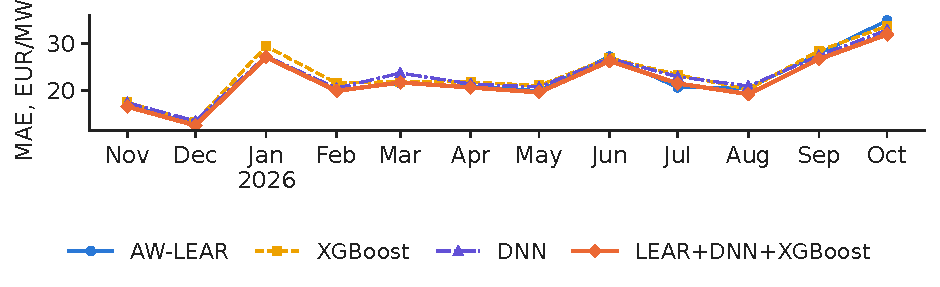
\includegraphics[width=\textwidth,height=0.497\textheight,keepaspectratio]{charts/en/monthly_ml.pdf}\end{center}\vspace{-3mm}
\chartsource{Source: energy-charts.info (Fraunhofer ISE); Yahoo Finance (EUA). Data: test year 2025-11-01 to 2026-10-31.}
\vspace{0.5mm}
\begin{itemize}\setlength{\itemsep}{0pt}
  \item Alone, XGBoost and the DNN each beat AW-LEAR in only 3 months
    \begin{itemize}\setlength{\itemsep}{0pt}
      \item Averaged with it, in 10.
    \end{itemize}
  \item All models err more in the same months (January, June, October): the hard days are hard for everyone.
\end{itemize}
\par\vfill\manager{report accuracy month by month to the risk committee, not only the annual average.}\par\vspace{0.5mm}
\par\vfill\noindent{\scriptsize\color{FooterGray}(own computation, test year 1 Nov 2025 -- 31 Oct 2026)}\hfill\qlink{EMQA\_L7\_monthly\_ml}{Quantlets/L7/EMQA_L7_monthly_ml}\par\vspace{0.5mm}
\end{frame}

\begin{frame}{Compute cost: daily LEAR is the expensive model, ML costs minutes}
\small
\begin{center}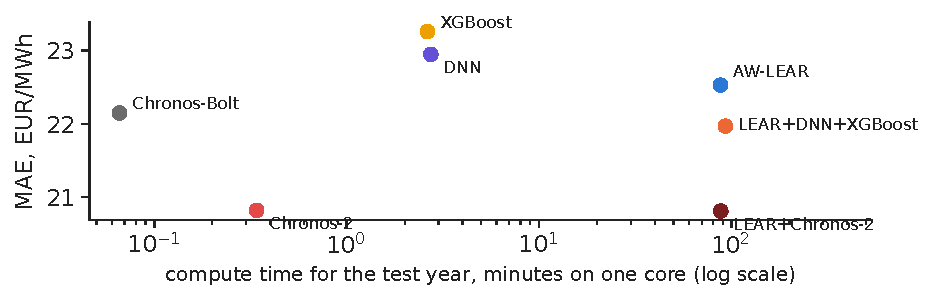
\includegraphics[width=\textwidth,height=0.580\textheight,keepaspectratio]{charts/en/cost_gain.pdf}\end{center}\vspace{-3mm}
\chartsource{Source: energy-charts.info (Fraunhofer ISE); Yahoo Finance (EUA). Data: test year 2025-11-01 to 2026-10-31; one processor core.}
\vspace{0.5mm}
\begin{itemize}\setlength{\itemsep}{0pt}
  \item Test year, one core: AW-LEAR 87.6 min (365 days $\times$ 3 windows $\times$ 24 h)
    \begin{itemize}\setlength{\itemsep}{0pt}
      \item XGBoost 2.6 min, DNN 2.7 min, Chronos-2 0.3 min
    \end{itemize}
  \item Hidden costs: the search (7.3 min), the pretraining of Chronos, the people who run the pipeline.
\end{itemize}
\par\vfill\manager{compare models on error per euro of total cost of ownership, not on error alone.}\par\vspace{0.5mm}
\par\vfill\noindent{\scriptsize\color{FooterGray}(own computation; times measured on one core of an 18-core laptop)}\hfill\qlink{EMQA\_L7\_cost\_gain}{Quantlets/L7/EMQA_L7_cost_gain}\par\vspace{0.5mm}
\end{frame}


\section{Explaining the forecasts}

\begin{frame}{Shapley values split each forecast into the contributions of its inputs}
\footnotesize
\intuition{The contribution of an input is its average effect when it is added to the model, over all orders in which the inputs could be added.}
\begin{columns}[T,onlytextwidth]
\begin{column}{0.53\textwidth}
\[ \phi_j=\sum_{S\not\ni j}\tfrac{|S|!\,(p-|S|-1)!}{p!}\big[v(S\cup\{j\})-v(S)\big] \]\vspace{-2mm}\[ \hat f(\mathbf x)=\phi_0+\textstyle\sum_{j}\phi_j \]{\footnotesize\begin{itemize}\setlength{\itemsep}{0pt}
  \item \textbf{\txtwhere}
    \begin{itemize}\setlength{\itemsep}{0pt}
      \item $\phi_j$ = SHapley Additive exPlanations (SHAP) value of input $j$
      \item $S$ = a subset of the other inputs
      \item $v(S)$ = expected forecast when only $S$ is known
      \item $\phi_0$ = average forecast
      \item $p$ = 20 inputs.
    \end{itemize}
\end{itemize}\par}
\end{column}
\begin{column}{0.44\textwidth}
\begin{itemize}\setlength{\itemsep}{1pt}
  \item \textbf{Why Shapley values}
    \begin{itemize}\setlength{\itemsep}{0pt}
      \item The only fair split in the game-theory sense; they add up exactly to the forecast
    \end{itemize}
  \item \textbf{On our data}
    \begin{itemize}\setlength{\itemsep}{0pt}
      \item XGBoost, 8\,760 test hours; largest gap between $\hat f$ and $\phi_0+\sum\phi_j$: 0.000009
      \item Past prices carry 69.3\% of the total contribution
    \end{itemize}
\end{itemize}
\end{column}
\end{columns}
\par\vfill\manager{ask for the explanation of each alarm, not only for a global ranking.}\par\vspace{0.5mm}
\par\vfill\noindent{\scriptsize\color{FooterGray}(Shapley, 1953; Lundberg et al., 2020, Nat.\ Mach.\ Intell.)}\hfill\tryit{notebook \S6}\par\vspace{0.5mm}
\end{frame}

\begin{frame}{What drives the trees: yesterday's price at the same hour}
\small
\begin{center}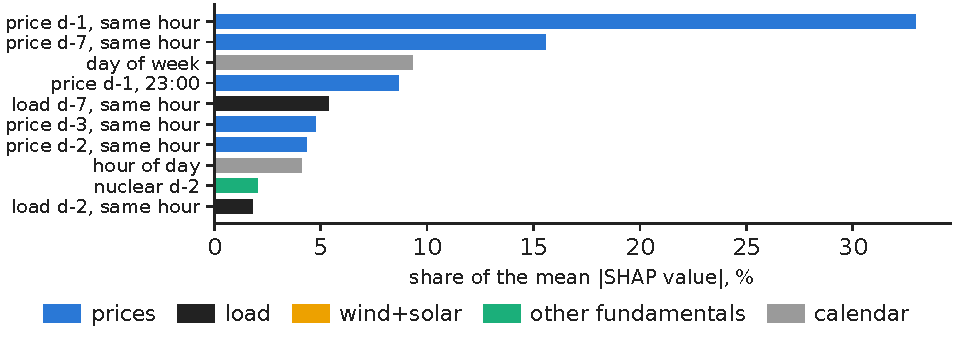
\includegraphics[width=\textwidth,height=0.486\textheight,keepaspectratio]{charts/en/shap_global.pdf}\end{center}\vspace{-3mm}
\chartsource{Source: energy-charts.info (Fraunhofer ISE); Yahoo Finance (EUA). Data: test year 2025-11-01 to 2026-10-31, 8760 hours.}
\vspace{0.5mm}
\begin{itemize}\setlength{\itemsep}{0pt}
  \item Top inputs: price $d-1$ same hour 32.9\%, price $d-7$ same hour 15.6\%, day of week 9.3\% of the mean $|\phi|$.
  \item Load 8.5\%, wind + solar 2.5\%: known only up to $d-2$, they are old news at gate closure.
\end{itemize}
\par\vfill\manager{buy better inputs first: the load and wind forecasts of the transmission system operator (TSO).}\par\vspace{0.5mm}
\par\vfill\noindent{\scriptsize\color{FooterGray}(own computation, test year 1 Nov 2025 -- 31 Oct 2026)}\hfill\qlink{EMQA\_L7\_shap\_global}{Quantlets/L7/EMQA_L7_shap_global}\par\vspace{0.5mm}
\end{frame}

\begin{frame}{Wind and solar lower the price only in the hours when they are large}
\small
\begin{center}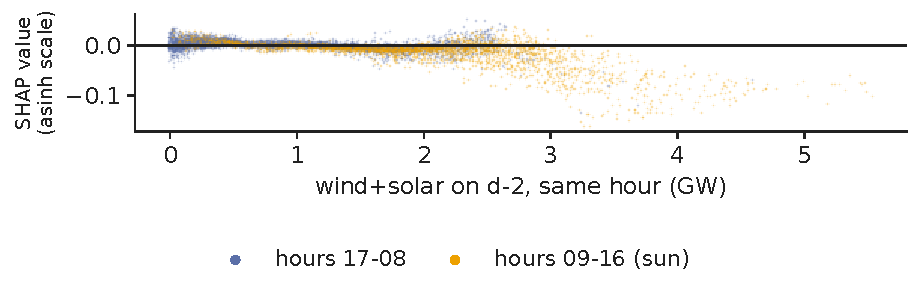
\includegraphics[width=\textwidth,height=0.487\textheight,keepaspectratio]{charts/en/shap_res.pdf}\end{center}\vspace{-3mm}
\chartsource{Source: energy-charts.info (Fraunhofer ISE); Yahoo Finance (EUA). Data: test year 2025-11-01 to 2026-10-31, 8760 hours.}
\vspace{0.5mm}
\begin{itemize}\setlength{\itemsep}{0pt}
  \item Each point is one test hour
    \begin{itemize}\setlength{\itemsep}{0pt}
      \item The more wind + solar on $d-2$ at that hour, the more negative its contribution (correlation \ensuremath{-}0.64)
    \end{itemize}
  \item The effect appears above about 2 gigawatts (GW): a threshold that a linear model cannot express.
\end{itemize}
\par\vfill\manager{a solar developer can read here the price discount that its own output helps to create.}\par\vspace{0.5mm}
\par\vfill\noindent{\scriptsize\color{FooterGray}(own computation, test year 1 Nov 2025 -- 31 Oct 2026)}\hfill\qlink{EMQA\_L7\_shap\_res}{Quantlets/L7/EMQA_L7_shap_res}\par\vspace{0.5mm}
\end{frame}

\begin{frame}{The neural network relies even more on yesterday's prices}
\small
\begin{center}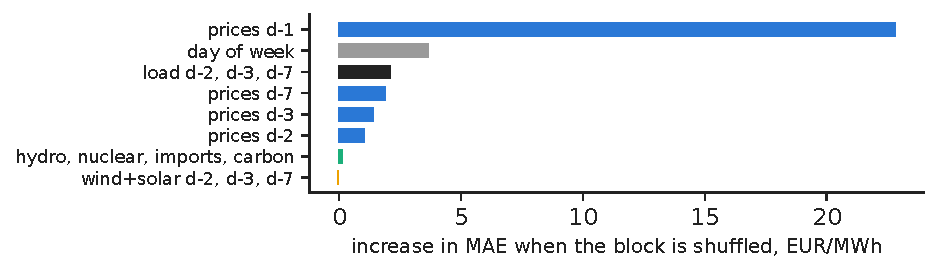
\includegraphics[width=\textwidth,height=0.469\textheight,keepaspectratio]{charts/en/perm_dnn.pdf}\end{center}\vspace{-3mm}
\chartsource{Source: energy-charts.info (Fraunhofer ISE); Yahoo Finance (EUA). Data: test year 2025-11-01 to 2026-10-31.}
\vspace{0.5mm}
\begin{itemize}\setlength{\itemsep}{0pt}
  \item Permutation importance $I_b$ = rise in MAE when block $b$ is shuffled across test days
    \begin{itemize}\setlength{\itemsep}{0pt}
      \item 5 permutations, valid for any model
    \end{itemize}
  \item Prices of $d-1$: +22.82 EUR/MWh
    \begin{itemize}\setlength{\itemsep}{0pt}
      \item Day of week +3.66, load +2.12, wind + solar \ensuremath{-}0.08
    \end{itemize}
\end{itemize}
\par\vfill\manager{monitor the price feed of $d-1$ first: the network fails without it.}\par\vspace{0.5mm}
\par\vfill\noindent{\scriptsize\color{FooterGray}(Breiman, 2001, Mach.\ Learn.; own computation)}\hfill\qlink{EMQA\_L7\_perm\_dnn}{Quantlets/L7/EMQA_L7_perm_dnn}\par\vspace{0.5mm}
\end{frame}

\begin{frame}{Energy finance uses machine learning widely but rarely explains it}
\footnotesize
\begin{columns}[T,onlytextwidth]
\begin{column}{0.52\textwidth}
\begin{itemize}\setlength{\itemsep}{1pt}
  \item \textbf{R.\ Clodnitchi, talk} (3 June 2026, \href{https://github.com/danpele/EMQA/blob/main/resources/aida2026/clodnitchi_ai_energy_finance_review.pdf}{slides})
    \begin{itemize}\setlength{\itemsep}{0pt}
      \item Systematic review of artificial intelligence (AI) in energy finance (Anagnoste et al., 2025, \textit{Energy Strategy Reviews})
      \item About 700 Web of Science articles screened, 232 peer-reviewed kept (2020--2025), on six pillars of energy finance
    \end{itemize}
  \item \textbf{Where AI is used} (share of papers using AI/ML)
    \begin{itemize}\setlength{\itemsep}{0pt}
      \item Pricing mechanisms 100\%, energy derivatives 100\%, energy and financial markets 97.5\%, risk management 93.0\%
      \item Green finance 60.4\%; corporate finance of energy firms 0\% (panel econometrics only)
    \end{itemize}
\end{itemize}
\end{column}
\begin{column}{0.45\textwidth}
\begin{itemize}\setlength{\itemsep}{1pt}
  \item \textbf{What is missing}
    \begin{itemize}\setlength{\itemsep}{0pt}
      \item Explainable AI: 19.6\% of the derivatives papers, 0--5\% in the other pillars
      \item Neural networks dominate: 88.2\% of the derivatives papers, 72.1\% in risk management
      \item Proposed next step: explainable AI and causal machine learning for regulators and policy evaluation
    \end{itemize}
  \item \textbf{Link with this lecture}
    \begin{itemize}\setlength{\itemsep}{0pt}
      \item The SHAP and permutation charts of this section are the kind of explanation the review finds rare
    \end{itemize}
\end{itemize}
\end{column}
\end{columns}
\par\vfill\manager{ask for the explanation together with the forecast: regulators and boards will ask for it.}\par\vspace{0.5mm}
\par\vfill\noindent{\scriptsize\color{FooterGray}(AIDA 2026 slides, Bucharest; paper: \href{https://doi.org/10.1016/j.esr.2025.101833}{Anagnoste et al., 2025, ESR})}\par\vspace{0.5mm}
\end{frame}


\section{Spikes, negative prices and a case study}

\begin{frame}{Spikes come in the evening, negative prices at midday}
\small
\begin{center}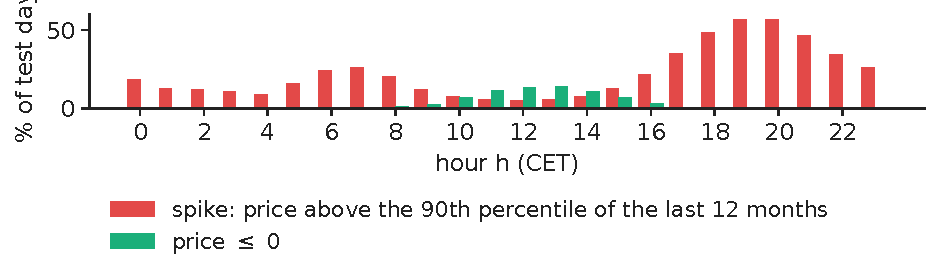
\includegraphics[width=\textwidth,height=0.457\textheight,keepaspectratio]{charts/en/events_hour.pdf}\end{center}\vspace{-3mm}
\chartsource{Source: energy-charts.info (Fraunhofer ISE): OPCOM prices. Data: test year 2025-11-01 to 2026-10-31.}
\vspace{0.5mm}
\begin{itemize}\setlength{\itemsep}{0pt}
  \item \textbf{Spike}: price above $\theta$, the 90th percentile of the hourly prices of the 12 months before the delivery month
    \begin{itemize}\setlength{\itemsep}{0pt}
      \item $\theta$ from 166.8 to 202.4 EUR/MWh; 22.1\% of test hours are spikes, most at 19:00 (57.0\% of days)
    \end{itemize}
  \item \textbf{Price $\leq$ 0}: 255 hours on 53 days of the test year, mostly around 13:00.
\end{itemize}
\par\vfill\manager{a battery charges at midday and discharges at 19:00--20:00: the two events are its business model.}\par\vspace{0.5mm}
\par\vfill\noindent{\scriptsize\color{FooterGray}(own computation, test year 1 Nov 2025 -- 31 Oct 2026)}\hfill\qlink{EMQA\_L7\_events\_hour}{Quantlets/L7/EMQA_L7_events_hour}\par\vspace{0.5mm}
\end{frame}

\begin{frame}{Spike classifiers: a good price forecast already detects spikes}
\footnotesize
\intuition{A classifier gives the probability that an hour is a spike; we judge how well it ranks the hours and how honest its probabilities are.}
\begin{columns}[T,onlytextwidth]
\begin{column}{0.56\textwidth}
\[ \hat\pi_{d,h}=\Pr\big(P_{d,h}>\theta_d\mid\mathbf x_{d,h}\big) \]\vspace{-2mm}\[ \text{Brier}=\frac{1}{n}\sum_{d,h}\big(\hat\pi_{d,h}-S_{d,h}\big)^2 \]{\footnotesize\begin{itemize}\setlength{\itemsep}{0pt}
  \item \textbf{\txtwhere}
    \begin{itemize}\setlength{\itemsep}{0pt}
      \item $S_{d,h}$ = 1 if the hour is a spike, 0 otherwise
      \item Precision = share of alerts that were spikes
      \item Recall = share of spikes that got an alert
      \item F1 = their harmonic mean
      \item Area under the curve (AUC) = probability that a spike hour gets a higher score than a normal hour.
    \end{itemize}
\end{itemize}\par}
\end{column}
\begin{column}{0.41\textwidth}
\begin{itemize}\setlength{\itemsep}{1pt}
  \item \textbf{On our data}: XGBoost and logistic classifiers, refitted monthly
    \begin{itemize}\setlength{\itemsep}{0pt}
      \item Spikes in 22.1\% of test hours, 14.3\% in the last training sample
      \item Brier score: XGBoost 0.072; constant share of spikes 0.172
    \end{itemize}
  \item \textbf{Benchmarks}
    \begin{itemize}\setlength{\itemsep}{0pt}
      \item Persistence: share of spikes at the same hour in the last 7 days
      \item The AW-LEAR price forecast itself, compared with $\theta$
    \end{itemize}
\end{itemize}
\end{column}
\end{columns}
\par\vfill\manager{judge an alert by its probabilities, not only by how many spikes it catches.}\par\vspace{0.5mm}
\par\vfill\noindent{\scriptsize\color{FooterGray}(Brier, 1950; Fawcett, 2006)}\hfill\tryit{notebook \S7}\par\vspace{0.5mm}
\end{frame}

\begin{frame}{Alerts on the test year: AW-LEAR matches a dedicated classifier}
\small
\begin{center}{\footnotesize\renewcommand{\arraystretch}{1.25}\setlength{\tabcolsep}{4pt}
\begin{tabular}{@{}lrrrrrrr@{}}\toprule
Model & AUC & Precision & Recall & F1 & Brier & AUC & F1 \\ \midrule
XGBoost & 0.953 & 0.826 & 0.685 & 0.749 & 0.072 & 0.980 & 0.571 \\
Logistic regression & 0.953 & 0.847 & 0.641 & 0.730 & 0.072 & 0.980 & 0.581 \\
Persistence, 7 days & 0.918 & 0.761 & 0.681 & 0.719 & 0.083 & 0.847 & 0.205 \\
AW-LEAR forecast $>\theta$ & 0.959 & 0.851 & 0.733 & 0.788 & -- & 0.983 & 0.558 \\
\bottomrule\end{tabular}}\end{center}
\par\vspace{0.5mm}{\scriptsize \begin{itemize}\setlength{\itemsep}{0pt}
  \item Columns 2--6: spikes (1\,938 hours); columns 7--8: prices $\leq$ 0 (255 hours). Alert when probability $>$ 0.5; AW-LEAR: alert when its price forecast exceeds $\theta$ (or is $\leq$ 0).
  \item For negative prices, XGBoost catches only 0.467 of the events at threshold 0.5: these hours are rare and depend on tomorrow's weather.
\end{itemize}}
\par\vfill\manager{buy a spike-alert service only if it beats the spike signal already hidden in your price forecast.}\par\vspace{0.5mm}
\par\vfill\noindent{\scriptsize\color{FooterGray}(own computation, test year 1 Nov 2025 -- 31 Oct 2026)}\hfill\tryit{notebook \S7}\par\vspace{0.5mm}
\end{frame}

\begin{frame}{Persistence detects spikes, but not negative prices}
\small
\begin{center}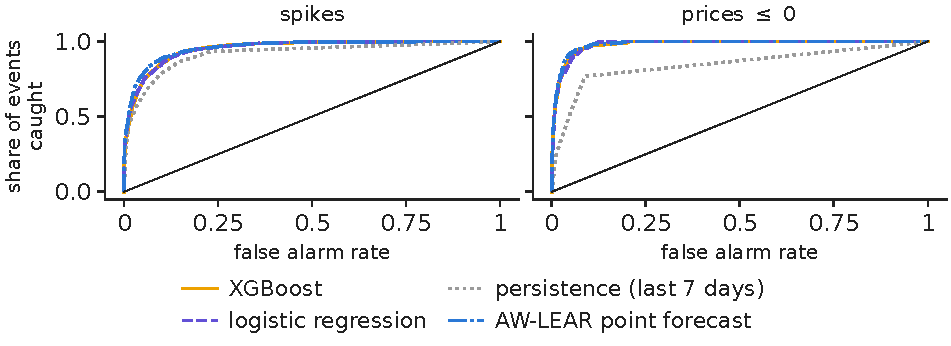
\includegraphics[width=\textwidth,height=0.556\textheight,keepaspectratio]{charts/en/roc.pdf}\end{center}\vspace{-3mm}
\chartsource{Source: energy-charts.info (Fraunhofer ISE); Yahoo Finance (EUA). Data: test year 2025-11-01 to 2026-10-31, 8760 hours.}
\vspace{0.5mm}
\begin{itemize}\setlength{\itemsep}{0pt}
  \item Receiver operating characteristic (ROC) curves
    \begin{itemize}\setlength{\itemsep}{0pt}
      \item Spikes: AUC from 0.918 (persistence) to 0.959 (AW-LEAR), since the evening spike repeats day after day.
    \end{itemize}
  \item Negative prices: persistence 0.847 against 0.980 for XGBoost
    \begin{itemize}\setlength{\itemsep}{0pt}
      \item They depend on tomorrow's sun and wind, not on yesterday.
    \end{itemize}
\end{itemize}
\par\vfill\noindent{\scriptsize\color{FooterGray}(own computation, test year 1 Nov 2025 -- 31 Oct 2026)}\hfill\qlink{EMQA\_L7\_roc}{Quantlets/L7/EMQA_L7_roc}\par\vspace{0.5mm}
\end{frame}

\begin{frame}{Cost--loss rule: act when the spike probability exceeds C/L}
\small
\begin{center}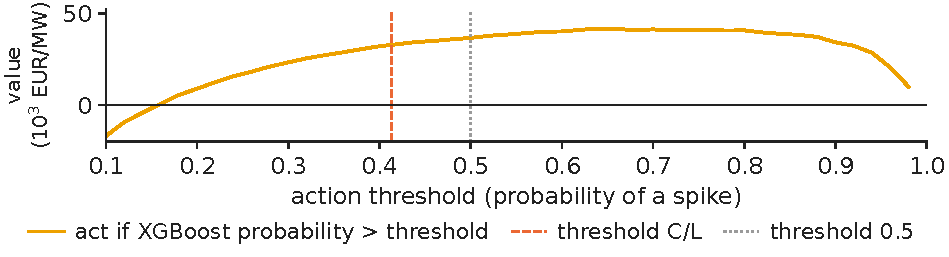
\includegraphics[width=\textwidth,height=0.442\textheight,keepaspectratio]{charts/en/decision.pdf}\end{center}\vspace{-3mm}
\chartsource{Source: energy-charts.info (Fraunhofer ISE); Yahoo Finance (EUA). Data: test year 2025-11-01 to 2026-10-31; 1 MW of flexible load.}
\vspace{0.5mm}
\begin{itemize}\setlength{\itemsep}{0pt}
  \item \textbf{Rule}: act if $\hat\pi_{d,h}>C/\bar L$ = 30/72.5 = 0.414
    \begin{itemize}\setlength{\itemsep}{0pt}
      \item C = cost of acting = 30 EUR/MWh (assumed): moving 1 MWh out of an alerted hour earns $P_{d,h}-\theta_d-C$
      \item $\bar L$ = cost of a missed spike = mean excess over $\theta$ in the validation year
    \end{itemize}
  \item Value per MW and year: 33.0 thousand EUR at C/L, 11.8 with persistence, 62.4 with perfect foresight.
\end{itemize}
\par\vfill\manager{set the threshold from your costs, not from hindsight (best threshold ex post: 0.64).}\par\vspace{0.5mm}
\par\vfill\noindent{\scriptsize\color{FooterGray}(Murphy, 1977, MWR; own computation)}\hfill\qlink{EMQA\_L7\_decision}{Quantlets/L7/EMQA_L7_decision}\par\vspace{0.5mm}
\end{frame}

\begin{frame}{Case study, 30 Jun 2026: every model saw the spike, none its size}
\small
\begin{center}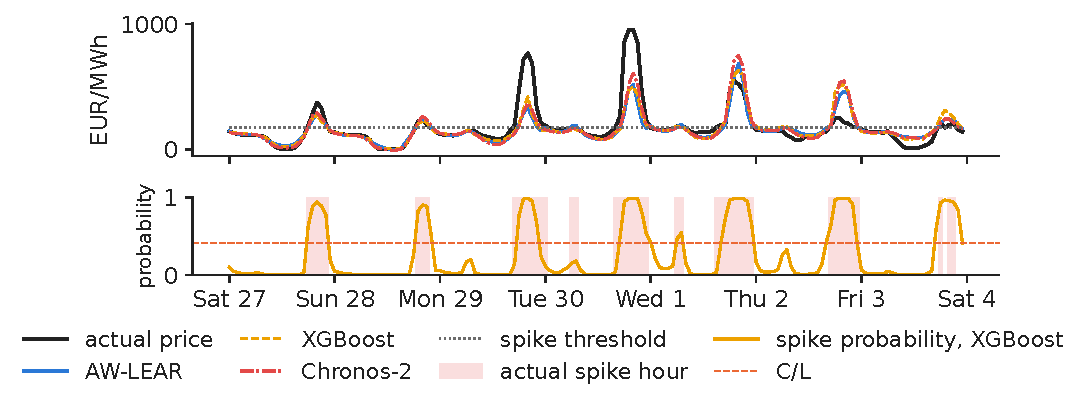
\includegraphics[width=\textwidth,height=0.502\textheight,keepaspectratio]{charts/en/case_week.pdf}\end{center}\vspace{-3mm}
\chartsource{Source: energy-charts.info (Fraunhofer ISE); Yahoo Finance (EUA). Data: 2026-06-27 to 2026-07-03, hourly.}
\vspace{0.5mm}
\begin{itemize}\setlength{\itemsep}{0pt}
  \item \textbf{Hour 20:00 CET}: 954.59 EUR/MWh, the highest price of the test year
    \begin{itemize}\setlength{\itemsep}{0pt}
      \item Forecasts: AW-LEAR 520, XGBoost 499, DNN 614, Chronos-2 607; spike probability 0.992
    \end{itemize}
  \item In that week: 47 spike hours, 45 alerts at C/L, 39 of them correct.
\end{itemize}
\par\vfill\manager{the probability says whether to act, the point forecast how much.}\par\vspace{0.5mm}
\par\vfill\noindent{\scriptsize\color{FooterGray}(own computation; Romanian day-ahead prices)}\hfill\qlink{EMQA\_L7\_case\_week}{Quantlets/L7/EMQA_L7_case_week}\par\vspace{0.5mm}
\end{frame}

\begin{frame}{Case study: the trees followed the extreme evening of the day before}
\small
\begin{center}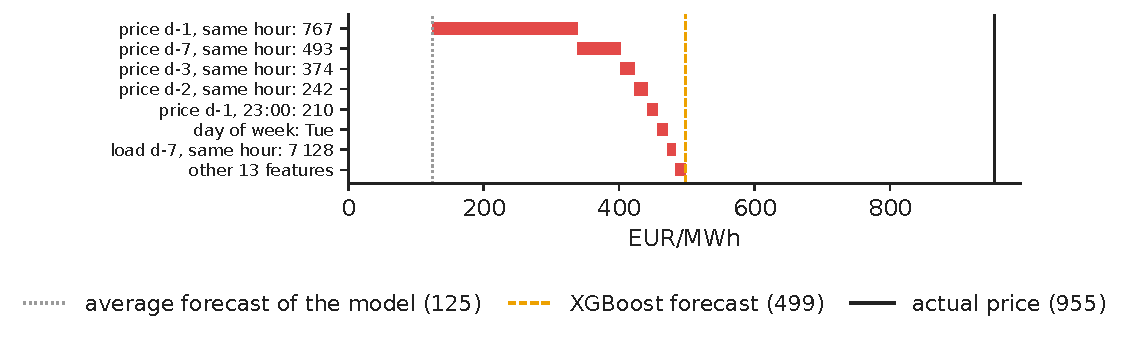
\includegraphics[width=\textwidth,height=0.470\textheight,keepaspectratio]{charts/en/shap_local.pdf}\end{center}\vspace{-3mm}
\chartsource{Source: energy-charts.info (Fraunhofer ISE); Yahoo Finance (EUA). Data: 2026-06-30, hour 20:00 CET; contributions rescaled to EUR/MWh (Appendix C).}
\vspace{0.5mm}
\begin{itemize}\setlength{\itemsep}{0pt}
  \item From 125 (model average) to 499 EUR/MWh: price of $d-1$, same hour, \ensuremath{+}213
    \begin{itemize}\setlength{\itemsep}{0pt}
      \item Price of $d-7$ \ensuremath{+}64.
    \end{itemize}
  \item Trees cannot go above the prices stored in their leaves: extremes are capped.
\end{itemize}
\par\vfill\manager{show the board this breakdown for every large alert.}\par\vspace{0.5mm}
\par\vfill\noindent{\scriptsize\color{FooterGray}(own computation; SHAP values in EUR/MWh, Appendix C)}\hfill\qlink{EMQA\_L7\_shap\_local}{Quantlets/L7/EMQA_L7_shap_local}\par\vspace{0.5mm}
\end{frame}

\begin{frame}{Our group on spike early warning: the paper and our replication}
\footnotesize
\begin{itemize}\setlength{\itemsep}{1pt}
  \item \textbf{What the paper did} (Andrei, Pele, Cramer, Amza \& Diaconu, 2026)
    \begin{itemize}\setlength{\itemsep}{0pt}
      \item Data: 5,000 hours of the Romanian day-ahead market in 2024, with load, renewable and fuel data; spike = price above the 90th percentile
      \item Method: random forests and XGBoost explained with SHAP; an early-warning score built from the thresholds of several indicators
      \item Result: the previous price and the residual load forecast are the main drivers of spikes
    \end{itemize}
  \item \textbf{Our replication} (case study C7, gate-closure information only)
    \begin{itemize}\setlength{\itemsep}{0pt}
      \item Test period Jul 2025 -- Oct 2026; spikes in 22.1\% of hours (training: 10.0\%)
      \item XGBoost AUC 0.946; top drivers: yesterday's and last week's price at the same hour, as on the previous slides
    \end{itemize}
\end{itemize}
\par\vspace{0.5mm}{\scriptsize \begin{itemize}\setlength{\itemsep}{0pt}
  \item Paper results as stated in the paper; replication numbers computed by the C7 case notebook on our data.
\end{itemize}}
\par\vfill\manager{a residual-load forecast is the input that a spike model needs most and that our public data lack.}\par\vspace{0.5mm}
\par\vfill\noindent{\scriptsize\color{FooterGray}(Andrei, Pele, Cramer, Amza \& Diaconu, 2026, PICBE; case study C7)}\par\vspace{0.5mm}
\end{frame}


\section{Pitfalls that flatter a model}

\begin{frame}{Look-ahead: two invalid evaluations flatter XGBoost}
\small
\begin{center}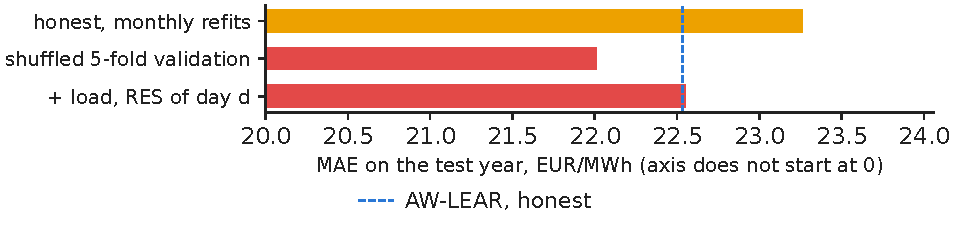
\includegraphics[width=\textwidth,height=0.428\textheight,keepaspectratio]{charts/en/pit_leak.pdf}\end{center}\vspace{-3mm}
\chartsource{Source: energy-charts.info (Fraunhofer ISE); Yahoo Finance (EUA). Data: test year 2025-11-01 to 2026-10-31.}
\vspace{0.5mm}
\begin{itemize}\setlength{\itemsep}{0pt}
  \item \textbf{Shuffled 5-fold cross-validation}: future days end up in the training sample
    \begin{itemize}\setlength{\itemsep}{0pt}
      \item MAE 22.01 instead of 23.26: 5.4\% better, on paper only
    \end{itemize}
  \item \textbf{Load and renewable energy sources (RES) of day $d$ as inputs}: unknown at 12:00 on $d-1$
    \begin{itemize}\setlength{\itemsep}{0pt}
      \item MAE 22.55, an apparent gain of 3.1\%: the most that perfect forecasts of these inputs could add
    \end{itemize}
\end{itemize}
\par\vfill\manager{ask every vendor for a walk-forward test with each input time-stamped at gate closure.}\par\vspace{0.5mm}
\par\vfill\noindent{\scriptsize\color{FooterGray}(Bergmeir \& Benítez, 2012, Inf.\ Sci.; own computation)}\hfill\qlink{EMQA\_L7\_pit\_leak}{Quantlets/L7/EMQA_L7_pit_leak}\par\vspace{0.5mm}
\end{frame}

\begin{frame}{Data snooping: choosing on the test year fakes a win over LEAR}
\small
\begin{center}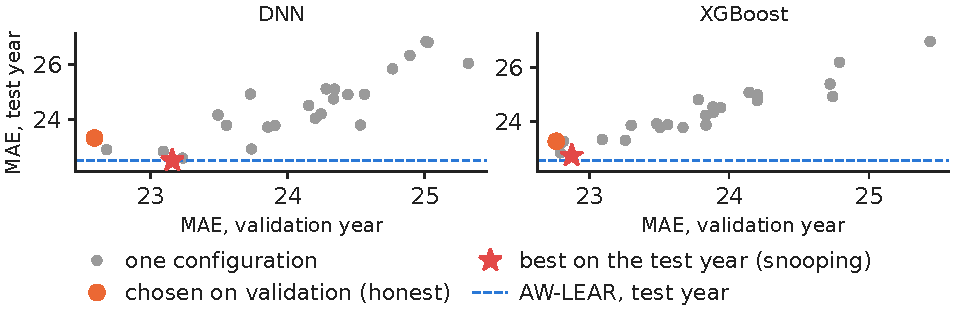
\includegraphics[width=\textwidth,height=0.506\textheight,keepaspectratio]{charts/en/snooping.pdf}\end{center}\vspace{-3mm}
\chartsource{Source: energy-charts.info (Fraunhofer ISE); Yahoo Finance (EUA). Data: validation and test year 2025-11-01 to 2026-10-31.}
\vspace{0.5mm}
\begin{itemize}\setlength{\itemsep}{0pt}
  \item Honest DNN (chosen on validation, 1 seed): MAE 23.34
    \begin{itemize}\setlength{\itemsep}{0pt}
      \item Best of 25 settings on the test year: 22.52, just below AW-LEAR (22.53).
    \end{itemize}
  \item Validation works, but not perfectly: Spearman rank correlation 0.86 (DNN), 0.94 (XGBoost).
\end{itemize}
\par\vfill\manager{ask how many models were tried: the more trials, the more the best one flatters.}\par\vspace{0.5mm}
\par\vfill\noindent{\scriptsize\color{FooterGray}(White, 2000, Econometrica; own computation)}\hfill\qlink{EMQA\_L7\_snooping}{Quantlets/L7/EMQA_L7_snooping}\par\vspace{0.5mm}
\end{frame}

\begin{frame}{The best of many models must be tested against the benchmark}
\footnotesize
\begin{columns}[T,onlytextwidth]
\begin{column}{0.44\textwidth}
\vspace{-2mm}\[ \mathrm{RC}_n=\max_{k=1,\dots,m}\sqrt{n}\,\bar d_k,\qquad \bar d_k=\frac1n\sum_{t=1}^{n}d_{k,t} \]{\footnotesize\begin{itemize}\setlength{\itemsep}{0pt}
  \item \textbf{\txtwhere}
    \begin{itemize}\setlength{\itemsep}{0pt}
      \item $d_{k,t}$ = benchmark loss minus loss of model $k$ on day $t$
      \item $H_0$: $E(d_{k,t})\le 0$ for all $k$
      \item Critical value: joint bootstrap of $(d_{1,t},\dots,d_{m,t})$, which keeps the correlation between models.
    \end{itemize}
\end{itemize}\par}\begin{itemize}\setlength{\itemsep}{1pt}
  \item \textbf{Why}: for $m$ independent 5\% tests, P(at least one false win) = $1-0.95^m$: 0.401 ($m$ = 10), 0.994 ($m$ = 100).
\end{itemize}
\end{column}
\begin{column}{0.53\textwidth}
\begin{itemize}\setlength{\itemsep}{1pt}
  \item \textbf{C.-M.\ Kuan, 4 June 2026} (\href{https://github.com/danpele/EMQA/blob/main/resources/aida2026/kuan_multiple_inequality_testing.pdf}{slides})
    \begin{itemize}\setlength{\itemsep}{0pt}
      \item Reality Check (RC), White (2000): conservative, poor models added to the set reduce its power (Hansen, 2005)
      \item Superior predictive ability (SPA) test, Hansen (2005): recentres the poor models, more powerful
      \item Step-RC (Romano \& Wolf, 2005), Step-SPA (Hsu, Hsu \& Kuan, 2010): name the winners, familywise error rate (FWER) under control
    \end{itemize}
  \item \textbf{On our data}
    \begin{itemize}\setlength{\itemsep}{0pt}
      \item The best of 25 DNN settings on the test year is just below AW-LEAR: the selection RC and SPA correct for
    \end{itemize}
\end{itemize}
\end{column}
\end{columns}
\par\vfill\manager{when shown the best of many models, ask for an RC or SPA p-value against your benchmark.}\par\vspace{0.5mm}
\par\vfill\noindent{\scriptsize\color{FooterGray}(AIDA 2026 slides; papers: \href{https://doi.org/10.1111/1468-0262.00152}{White, 2000}; \href{https://doi.org/10.1198/073500105000000063}{Hansen, 2005}; \href{https://doi.org/10.1111/j.1468-0262.2005.00615.x}{Romano \& Wolf, 2005}; \href{https://doi.org/10.1016/j.jempfin.2010.01.001}{Hsu et al., 2010})}\par\vspace{0.5mm}
\end{frame}

\begin{frame}{Retraining: a model frozen for a year loses 4.2\%}
\small
\begin{center}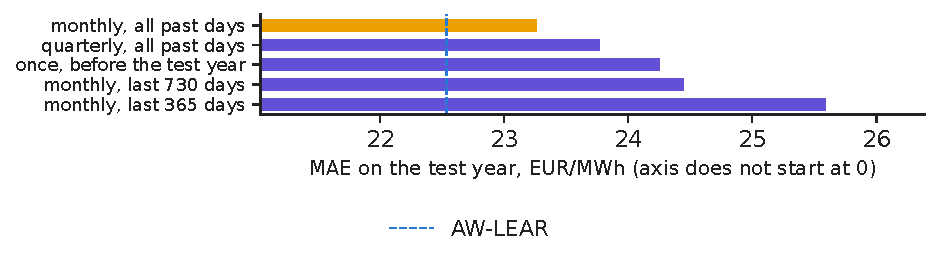
\includegraphics[width=\textwidth,height=0.450\textheight,keepaspectratio]{charts/en/pit_retrain.pdf}\end{center}\vspace{-3mm}
\chartsource{Source: energy-charts.info (Fraunhofer ISE); Yahoo Finance (EUA). Data: test year 2025-11-01 to 2026-10-31.}
\vspace{0.5mm}
\begin{itemize}\setlength{\itemsep}{0pt}
  \item Fitted once, before the test year: MAE 24.25
    \begin{itemize}\setlength{\itemsep}{0pt}
      \item The loss grows with time (+0.15 EUR/MWh in the first 3 months, +3.70 in the last 3).
    \end{itemize}
  \item A short rolling window (365 days, MAE 25.59) is worse than the whole history: the trees need many past spikes to learn from.
\end{itemize}
\par\vfill\manager{put the monthly refit in the operating calendar, with an owner, like any other control.}\par\vspace{0.5mm}
\par\vfill\noindent{\scriptsize\color{FooterGray}(own computation, test year 1 Nov 2025 -- 31 Oct 2026)}\hfill\qlink{EMQA\_L7\_pit\_retrain}{Quantlets/L7/EMQA_L7_pit_retrain}\par\vspace{0.5mm}
\end{frame}

\begin{frame}{Leakage self-check: deleting the future changes no forecast}
\footnotesize
\begin{columns}[T,onlytextwidth]
\begin{column}{0.52\textwidth}
\begin{itemize}\setlength{\itemsep}{1pt}
  \item \textbf{The test}
    \begin{itemize}\setlength{\itemsep}{0pt}
      \item For the first day of each of the 12 test months, all data after 12:00 on $d-1$ are deleted, then replaced by 10\,000 EUR/MWh
      \item XGBoost, the DNN and the spike classifier are refitted and must give the same forecasts
    \end{itemize}
  \item \textbf{Result}
    \begin{itemize}\setlength{\itemsep}{0pt}
      \item Trees and classifier: identical; DNN: differences below 0.001 EUR/MWh (rounding in parallel arithmetic)
      \item Chronos: the context is built only from days before day $d$, checked in the code
    \end{itemize}
\end{itemize}
\end{column}
\begin{column}{0.45\textwidth}
\begin{itemize}\setlength{\itemsep}{1pt}
  \item \textbf{Checklist before trusting a model}
    \begin{itemize}\setlength{\itemsep}{0pt}
      \item Every input time-stamped at gate closure
      \item Settings chosen on a validation year
      \item One test year, opened once, with DM tests against LEAR
      \item Monthly refits and a perturbation test like this one
    \end{itemize}
\end{itemize}
\end{column}
\end{columns}
\par\vfill\manager{make this check part of every model review, for statistical and machine-learning models alike.}\par\vspace{0.5mm}
\par\vfill\noindent{\scriptsize\color{FooterGray}(Lecture 2; Lago et al., 2021, APEN)}\hfill\tryit{notebook \S10}\par\vspace{0.5mm}
\end{frame}

\section*{Wrap-up}

\begin{frame}{Quiz 1: a perfect backtest}
\small
\begin{itemize}
  \item A start-up shows a neural network with rMAE 0.70 on Romania, tested with shuffled 5-fold cross-validation
    \begin{itemize}\setlength{\itemsep}{0pt}
      \item What do you ask for?
    \end{itemize}
\end{itemize}
\vspace{2mm}
\begin{exampleblock}{Answer}
\begin{itemize}
  \item A walk-forward test on one untouched year, with inputs known at 12:00 on $d-1$: on our data, shuffling alone made XGBoost look 5.4\% better.
\end{itemize}
\end{exampleblock}
\end{frame}

\begin{frame}{Quiz 2: which model to deploy}
\small
\begin{itemize}
  \item Chronos-2 has the lowest MAE of the single models
    \begin{itemize}\setlength{\itemsep}{0pt}
      \item AW-LEAR + Chronos-2 has the same MAE
      \item Which do you deploy?
    \end{itemize}
\end{itemize}
\vspace{2mm}
\begin{exampleblock}{Answer}
\begin{itemize}
  \item The combination: same accuracy (DM $p$ = 0.491), but if the pretrained model degrades or becomes unavailable, LEAR still carries half of the forecast.
\end{itemize}
\end{exampleblock}
\end{frame}

\begin{frame}{Quiz 3: reading SHAP}
\small
\begin{itemize}
  \item Load has a small SHAP share (8.5\%)
    \begin{itemize}\setlength{\itemsep}{0pt}
      \item Can we conclude that load does not affect the price?
    \end{itemize}
\end{itemize}
\vspace{2mm}
\begin{exampleblock}{Answer}
\begin{itemize}
  \item No: SHAP explains the model, not the market
    \begin{itemize}\setlength{\itemsep}{0pt}
      \item Load enters only with its $d-2$ value, already reflected in yesterday's price.
    \end{itemize}
\end{itemize}
\end{exampleblock}
\end{frame}

\begin{frame}{Quiz 4: an alert threshold}
\small
\begin{itemize}
  \item Moving 1 MWh costs you 60 EUR instead of 30
    \begin{itemize}\setlength{\itemsep}{0pt}
      \item How does the alert threshold change?
    \end{itemize}
\end{itemize}
\vspace{2mm}
\begin{exampleblock}{Answer}
\begin{itemize}
  \item It doubles: C/L rises from 0.414 to about twice that value, so you act only on the more certain spikes.
\end{itemize}
\end{exampleblock}
\end{frame}

\begin{frame}{Quiz 5: retraining}
\small
\begin{itemize}
  \item Your data team proposes to train the model once a year to save effort
    \begin{itemize}\setlength{\itemsep}{0pt}
      \item What does the test year say?
    \end{itemize}
\end{itemize}
\vspace{2mm}
\begin{exampleblock}{Answer}
\begin{itemize}
  \item A model frozen for the year was 4.2\% less accurate, and the gap widened in the last months
    \begin{itemize}\setlength{\itemsep}{0pt}
      \item A monthly refit of XGBoost takes about 13 seconds.
    \end{itemize}
\end{itemize}
\end{exampleblock}
\end{frame}

\begin{frame}{Wrap-up}
\small
\vspace{-2mm}\begin{multicols}{2}\scriptsize\tableofcontents\end{multicols}
\begin{itemize}\setlength{\itemsep}{1pt}
  \item Tuned, the DNN and XGBoost improve on Lecture 2 but do not beat AW-LEAR alone
    \begin{itemize}\setlength{\itemsep}{0pt}
      \item Averaged with it, they do.
    \end{itemize}
  \item Chronos-2, with no training, is the most accurate single model (MAE 20.82, 7.6\% below AW-LEAR)
    \begin{itemize}\setlength{\itemsep}{0pt}
      \item Every model must be explained, validated and refitted.
    \end{itemize}
\end{itemize}
\end{frame}

\begin{frame}{Research from our group on machine learning for Romanian power prices}
\footnotesize
\begin{itemize}\setlength{\itemsep}{1pt}
  \item \textbf{Early warning of price spikes} (Andrei, Pele, Cramer, Amza \& Diaconu, 2026, PICBE): built an explainable artificial intelligence (AI) system for the Romanian day-ahead market
    \begin{itemize}\setlength{\itemsep}{0pt}
      \item The previous price and the residual load drive the spikes --- case study C7.
    \end{itemize}
  \item \textbf{Explaining price forecasts across horizons} (Andrei, Pele \& Cramer, 2026, PICBE): explained machine-learning forecasts of Romanian hourly prices and showed which drivers matter at each horizon and in each price regime.
  \item \textbf{Four generations of price models} (Andrei, Velev, Toma, Pele \& Lessmann, 2024, arXiv 2411.03372): compared four generations of forecasting methods for energy prices, from statistical models to deep learning, as a guide for choosing a model family.
  \item \textbf{Foundation models for tail risk} (Jheng, Tak, Găman, Mazurencu-Marinescu-Pele \& Pele, 2026, ECECSR): used pretrained foundation models, without retraining and with conformal calibration, to forecast extreme losses in Central and Eastern European markets.
\end{itemize}
\par\vspace{0.5mm}{\scriptsize \begin{itemize}\setlength{\itemsep}{0pt}
  \item Findings as stated in the papers; numbers on the other slides come from our own data.
\end{itemize}}
\par\vfill\noindent{\scriptsize\color{FooterGray}(Bucharest University of Economic Studies; Romanian Academy, Institute for Economic Forecasting)}\par\vspace{0.5mm}
\end{frame}

\begin{frame}{Want to learn more?}
\small
\begin{columns}[T,onlytextwidth]
\begin{column}{0.52\textwidth}
\begin{itemize}\setlength{\itemsep}{1pt}
  \item \textbf{epftoolbox}: the DNN and LEAR of Lago et al.\ (2021) with open benchmark data --- \href{https://github.com/jeslago/epftoolbox}{github.com/jeslago/epftoolbox}.
  \item \textbf{XGBoost} and \textbf{shap} documentation: \href{https://xgboost.readthedocs.io}{xgboost.readthedocs.io}, \href{https://shap.readthedocs.io}{shap.readthedocs.io}.
  \item \textbf{Chronos} foundation models: \href{https://github.com/amazon-science/chronos-forecasting}{github.com/amazon-science/chronos-forecasting}.
  \item \textbf{Interpretable Machine Learning} (C.\ Molnar), free online: \href{https://christophm.github.io/interpretable-ml-book/}{christophm.github.io}.
\end{itemize}
\end{column}
\begin{column}{0.45\textwidth}
\begin{itemize}\setlength{\itemsep}{1pt}
  \item \textbf{This course}: code, data, notebooks --- \href{https://github.com/danpele/EMQA}{github.com/danpele/EMQA}.
  \item \textbf{Case study C7} replicates the spike early-warning paper on our data.
  \item \textbf{Experiment yourself}: the notebook reproduces every chart and number of this lecture --- \href{\emqarepo/\emqanb}{notebooks/}.
\end{itemize}
\end{column}
\end{columns}
\end{frame}

\begin{frame}{References (1/4)}
\scriptsize
\begin{itemize}\setlength{\itemsep}{1pt}\scriptsize
\item Anagnoste, S., Andrei, A.-V., Bolovăneanu, V., Cepoi, C.-O., Clodnitchi, R., Cramer, A.-A., Grecu, R.-A., Lessmann, S., Pele, D.\,T., Petukhina, A.\ \& Strat, V.\,A.\ (2025). The role of AI in (re)shaping energy finance: A systematic literature review. \textit{Energy Strategy Reviews}, 61, 101833. \href{https://doi.org/10.1016/j.esr.2025.101833}{doi:10.1016/j.esr.2025.101833}
\item Andrei, A.-V., Pele, D.-T.\ \& Cramer, A.-A.\ (2026). Multi-horizon explainability in energy price forecasting: Disentangling market dynamics and renewable intermittency in Romania's liberalized electricity market. \textit{Proceedings of the International Conference on Business Excellence}, 20(1), 104--117. \href{https://doi.org/10.2478/picbe-2026-0014}{doi:10.2478/picbe-2026-0014}
\item Andrei, A.-V., Pele, D.-T., Cramer, A.-A., Amza, A.\ \& Diaconu, D.\ (2026). Explainable AI-based early warning system for electricity price spikes: Evidence from the Romanian market. \textit{Proceedings of the International Conference on Business Excellence}, 20(1), 4820--4836. \href{https://doi.org/10.2478/picbe-2026-0352}{doi:10.2478/picbe-2026-0352}
\item Andrei, A.-V., Velev, G., Toma, F.-M., Pele, D.\,T.\ \& Lessmann, S.\ (2024). Energy price modelling: A comparative evaluation of four generations of forecasting methods. \href{https://arxiv.org/abs/2411.03372}{arXiv:2411.03372}
\item Andrei, A.-V., Velev, G., Toma, F.-M., Pele, D.\,T.\ \& Lessmann, S.\ (2026). Energy price modelling: A comparative evaluation of four generations of forecasting methods. Talk, AIDA Conference, Bucharest University of Economic Studies, 3 June 2026. \href{https://github.com/danpele/EMQA/blob/main/resources/aida2026/andrei_ai4efin_benchmarking.pdf}{github.com/danpele/EMQA/resources/aida2026}
\item Ansari, A.\,F., Stella, L., Turkmen, C.\ et al.\ (2024). Chronos: Learning the language of time series. \textit{Transactions on Machine Learning Research}. \href{https://arxiv.org/abs/2403.07815}{arXiv:2403.07815}
\item Ansari, A.\,F., Shchur, O., Küken, J.\ et al.\ (2025). Chronos-2: From univariate to universal forecasting. \href{https://arxiv.org/abs/2510.15821}{arXiv:2510.15821}
\item Bates, J.\,M.\ \& Granger, C.\,W.\,J.\ (1969). The combination of forecasts. \textit{Journal of the Operational Research Society}, 20(4), 451--468. \href{https://doi.org/10.1057/jors.1969.103}{doi:10.1057/jors.1969.103}
\item Bergmeir, C.\ \& Benítez, J.\,M.\ (2012). On the use of cross-validation for time series predictor evaluation. \textit{Information Sciences}, 191, 192--213. \href{https://doi.org/10.1016/j.ins.2011.12.028}{doi:10.1016/j.ins.2011.12.028}
\end{itemize}
\end{frame}

\begin{frame}{References (2/4)}
\scriptsize
\begin{itemize}\setlength{\itemsep}{1pt}\scriptsize
\item Bergstra, J.\ \& Bengio, Y.\ (2012). Random search for hyper-parameter optimization. \textit{Journal of Machine Learning Research}, 13, 281--305. \href{https://jmlr.org/papers/v13/bergstra12a.html}{jmlr.org/papers/v13/bergstra12a.html}
\item Breiman, L.\ (2001). Random forests. \textit{Machine Learning}, 45(1), 5--32. \href{https://doi.org/10.1023/A:1010933404324}{doi:10.1023/A:1010933404324}
\item Brier, G.\,W.\ (1950). Verification of forecasts expressed in terms of probability. \textit{Monthly Weather Review}, 78(1), 1--3. \href{https://doi.org/10.1175/1520-0493(1950)078<0001:VOFEIT>2.0.CO;2}{doi:10.1175/1520-0493(1950)078\allowbreak<0001:VOFEIT>2.0.CO;2}
\item Chen, T.\ \& Guestrin, C.\ (2016). XGBoost: A scalable tree boosting system. \textit{Proceedings of the 22nd ACM SIGKDD Conference}, 785--794. \href{https://doi.org/10.1145/2939672.2939785}{doi:10.1145/2939672.2939785}
\item Clodnitchi, R.\ (2026). The role of AI in (re)shaping energy finance: A systematic literature review. Talk, AIDA Conference, Bucharest University of Economic Studies, 3 June 2026. \href{https://github.com/danpele/EMQA/blob/main/resources/aida2026/clodnitchi_ai_energy_finance_review.pdf}{github.com/danpele/EMQA/resources/aida2026}
\item Diebold, F.\,X.\ \& Mariano, R.\,S.\ (1995). Comparing predictive accuracy. \textit{Journal of Business \& Economic Statistics}, 13(3), 253--263. \href{https://doi.org/10.1080/07350015.1995.10524599}{doi:10.1080/07350015.1995.10524599}
\item Fawcett, T.\ (2006). An introduction to ROC analysis. \textit{Pattern Recognition Letters}, 27(8), 861--874. \href{https://doi.org/10.1016/j.patrec.2005.10.010}{doi:10.1016/j.patrec.2005.10.010}
\item Friedman, J.\,H.\ (2001). Greedy function approximation: A gradient boosting machine. \textit{Annals of Statistics}, 29(5), 1189--1232. \href{https://doi.org/10.1214/aos/1013203451}{doi:10.1214/aos/1013203451}
\item Hansen, P.\,R.\ (2005). A test for superior predictive ability. \textit{Journal of Business \& Economic Statistics}, 23(4), 365--380. \href{https://doi.org/10.1198/073500105000000063}{doi:10.1198/073500105000000063}
\end{itemize}
\end{frame}

\begin{frame}{References (3/4)}
\scriptsize
\begin{itemize}\setlength{\itemsep}{1pt}\scriptsize
\item Hastie, T., Tibshirani, R.\ \& Friedman, J.\ (2009). \textit{The Elements of Statistical Learning}, 2nd ed. Springer. \href{https://doi.org/10.1007/978-0-387-84858-7}{doi:10.1007/978-0-387-84858-7}
\item Hsu, P.-H., Hsu, Y.-C.\ \& Kuan, C.-M.\ (2010). Testing the predictive ability of technical analysis using a new stepwise test without data snooping bias. \textit{Journal of Empirical Finance}, 17(3), 471--484. \href{https://doi.org/10.1016/j.jempfin.2010.01.001}{doi:10.1016/j.jempfin.2010.01.001}
\item Jheng, S., Tak, R., Găman, Ș., Mazurencu-Marinescu-Pele, M.\ \& Pele, D.\,T.\ (2026). Can foundation models manage risk? Zero-shot VaR and ES forecasting with conformal calibration in CEE markets. \textit{Economic Computation and Economic Cybernetics Studies and Research}, 60(2), 267--290. \href{https://doi.org/10.24818/18423264/60.2.26.14}{doi:10.24818/18423264/60.2.26.14}
\item Kingma, D.\,P.\ \& Ba, J.\ (2015). Adam: A method for stochastic optimization. \textit{International Conference on Learning Representations}. \href{https://arxiv.org/abs/1412.6980}{arXiv:1412.6980}
\item Kuan, C.-M.\ (2026). Large-scale multiple inequality testing without data snooping bias. Keynote, AIDA Conference, Bucharest University of Economic Studies, 4 June 2026. \href{https://github.com/danpele/EMQA/blob/main/resources/aida2026/kuan_multiple_inequality_testing.pdf}{github.com/danpele/EMQA/resources/aida2026}
\item Lago, J., De Ridder, F.\ \& De Schutter, B.\ (2018). Forecasting spot electricity prices: Deep learning approaches and empirical comparison of traditional algorithms. \textit{Applied Energy}, 221, 386--405. \href{https://doi.org/10.1016/j.apenergy.2018.02.069}{doi:10.1016/j.apenergy.2018.02.069}
\item Lago, J., Marcjasz, G., De Schutter, B.\ \& Weron, R.\ (2021). Forecasting day-ahead electricity prices: A review of state-of-the-art algorithms, best practices and an open-access benchmark. \textit{Applied Energy}, 293, 116983. \href{https://doi.org/10.1016/j.apenergy.2021.116983}{doi:10.1016/j.apenergy.2021.116983}
\item Lundberg, S.\,M., Erion, G., Chen, H.\ et al.\ (2020). From local explanations to global understanding with explainable AI for trees. \textit{Nature Machine Intelligence}, 2(1), 56--67. \href{https://doi.org/10.1038/s42256-019-0138-9}{doi:10.1038/s42256-019-0138-9}
\item Marcjasz, G., Narajewski, M., Weron, R.\ \& Ziel, F.\ (2023). Distributional neural networks for electricity price forecasting. \textit{Energy Economics}, 125, 106843. \href{https://doi.org/10.1016/j.eneco.2023.106843}{doi:10.1016/j.eneco.2023.106843}
\end{itemize}
\end{frame}

\begin{frame}{References (4/4)}
\scriptsize
\begin{itemize}\setlength{\itemsep}{1pt}\scriptsize
\item Murphy, A.\,H.\ (1977). The value of climatological, categorical and probabilistic forecasts in the cost-loss ratio situation. \textit{Monthly Weather Review}, 105(7), 803--816. \href{https://doi.org/10.1175/1520-0493(1977)105<0803:TVOCCA>2.0.CO;2}{doi:10.1175/1520-0493(1977)105\allowbreak<0803:TVOCCA>2.0.CO;2}
\item Olivares, K.\,G., Challu, C., Marcjasz, G., Weron, R.\ \& Dubrawski, A.\ (2023). Neural basis expansion analysis with exogenous variables: Forecasting electricity prices with NBEATSx. \textit{International Journal of Forecasting}, 39(2), 884--900. \href{https://doi.org/10.1016/j.ijforecast.2022.03.001}{doi:10.1016/j.ijforecast.2022.03.001}
\item Romano, J.\,P.\ \& Wolf, M.\ (2005). Stepwise multiple testing as formalized data snooping. \textit{Econometrica}, 73(4), 1237--1282. \href{https://doi.org/10.1111/j.1468-0262.2005.00615.x}{doi:10.1111/j.1468-0262.2005.00615.x}
\item Shapley, L.\,S.\ (1953). A value for n-person games. In \textit{Contributions to the Theory of Games II}, 307--317. Princeton University Press. \href{https://doi.org/10.1515/9781400881970-018}{doi:10.1515/9781400881970-018}
\item Srivastava, N., Hinton, G., Krizhevsky, A., Sutskever, I.\ \& Salakhutdinov, R.\ (2014). Dropout: A simple way to prevent neural networks from overfitting. \textit{Journal of Machine Learning Research}, 15, 1929--1958. \href{https://jmlr.org/papers/v15/srivastava14a.html}{jmlr.org/papers/v15/srivastava14a.html}
\item Weron, R.\ (2014). Electricity price forecasting: A review of the state-of-the-art with a look into the future. \textit{International Journal of Forecasting}, 30(4), 1030--1081. \href{https://doi.org/10.1016/j.ijforecast.2014.08.008}{doi:10.1016/j.ijforecast.2014.08.008}
\item Weron, R.\ (2026). Machine learning for electricity price forecasting. Keynote, AIDA Conference, Bucharest University of Economic Studies, 4 June 2026. \href{https://github.com/danpele/EMQA/blob/main/resources/aida2026/weron_ml_electricity_price_forecasting.pdf}{github.com/danpele/EMQA/resources/aida2026}
\item White, H.\ (2000). A reality check for data snooping. \textit{Econometrica}, 68(5), 1097--1126. \href{https://doi.org/10.1111/1468-0262.00152}{doi:10.1111/1468-0262.00152}
\end{itemize}
\end{frame}

\appendix

\section*{Appendix}

\begin{frame}{Appendix A: back-propagation and the Adam update}
\small
\begin{columns}[T,onlytextwidth]
\begin{column}{0.50\textwidth}
\[ \frac{\partial\mathcal L}{\partial W_2}=\boldsymbol\delta\,\mathbf z^{\top},\quad \boldsymbol\delta=\frac{\partial\mathcal L}{\partial\hat{\mathbf Y}} \]\[ \frac{\partial\mathcal L}{\partial W_1}=\big[(W_2^{\top}\boldsymbol\delta)\odot\phi'(\mathbf u)\big]\mathbf x^{\top} \]\begin{itemize}\setlength{\itemsep}{1pt}
  \item Chain rule, from the output back to the inputs
    \begin{itemize}\setlength{\itemsep}{0pt}
      \item For the absolute error $\partial|y-\hat y|/\partial\hat y=-\operatorname{sign}(y-\hat y)$.
    \end{itemize}
  \item $\mathbf u=W_1\mathbf x+\mathbf b_1$
    \begin{itemize}\setlength{\itemsep}{0pt}
      \item $\odot$ = element-wise product
      \item For softplus, $\phi'(u)=1/(1+e^{-u})$.
    \end{itemize}
\end{itemize}
\end{column}
\begin{column}{0.47\textwidth}
\[ m_k=\beta_1m_{k-1}+(1-\beta_1)g_k \]\[ v_k=\beta_2v_{k-1}+(1-\beta_2)g_k^2 \]\[ \theta_k=\theta_{k-1}-\eta\,\frac{m_k/(1-\beta_1^k)}{\sqrt{v_k/(1-\beta_2^k)}+\varepsilon} \]\begin{itemize}\setlength{\itemsep}{1pt}
  \item $g_k$ = gradient on mini-batch $k$
    \begin{itemize}\setlength{\itemsep}{0pt}
      \item $\beta_1=0.9$, $\beta_2=0.999$, $\varepsilon=10^{-8}$ (defaults)
      \item Each weight gets its own step size.
    \end{itemize}
  \item Weight decay adds $\lambda\theta$ to $g_k$ (a quadratic penalty, here $\lambda$ = $10^{-5}$).
\end{itemize}
\end{column}
\end{columns}
\par\vfill\noindent{\scriptsize\color{FooterGray}(Kingma \& Ba, 2015, ICLR; Hastie et al., 2009)}\par\vspace{0.5mm}
\end{frame}

\begin{frame}{Appendix B: why the optimal leaf value is $-G/(H+\lambda)$}
\small
\begin{columns}[T,onlytextwidth]
\begin{column}{0.52\textwidth}
\[ \ell\big(Y_i,F_{m-1}+f\big)\approx\ell_i+g_i f(\mathbf x_i)+\tfrac12h_i f(\mathbf x_i)^2 \]\[ \sum_{j}\Big[G_jw_j+\tfrac12(H_j+\lambda)w_j^2\Big]+\gamma J,\quad G_j=\textstyle\sum_{i\in R_j}g_i \]\[ w_j^{*}=-\frac{G_j}{H_j+\lambda},\qquad \text{score}=-\tfrac12\sum_j\frac{G_j^2}{H_j+\lambda}+\gamma J \]
\end{column}
\begin{column}{0.45\textwidth}
\begin{itemize}\setlength{\itemsep}{1pt}
  \item Second-order Taylor expansion of the loss around the current forecast
    \begin{itemize}\setlength{\itemsep}{0pt}
      \item $g_i$, $h_i$ = first and second derivatives
      \item $H_j$ = sum of $h_i$ in leaf $j$.
    \end{itemize}
  \item Within a leaf the objective is a parabola in $w_j$: setting its derivative to zero gives $w_j^*$.
  \item The split gain of the regression-tree slide is the score before the split minus the score after it.
  \item For the absolute error $h_i=0$
    \begin{itemize}\setlength{\itemsep}{0pt}
      \item XGBoost then sets the leaf values by a line search.
    \end{itemize}
\end{itemize}
\end{column}
\end{columns}
\par\vfill\noindent{\scriptsize\color{FooterGray}(Chen \& Guestrin, 2016, KDD)}\par\vspace{0.5mm}
\end{frame}

\begin{frame}{Appendix C: SHAP values in EUR/MWh}
\small
\begin{columns}[T,onlytextwidth]
\begin{column}{0.50\textwidth}
\[ \hat P=m+s\,\sinh\Big(\phi_0+\textstyle\sum_j\phi_j\Big),\qquad P_0=m+s\,\sinh\phi_0 \]\[ \phi_j^{\text{EUR}}=\phi_j\,\frac{\hat P-P_0}{\sum_k\phi_k}\ \Rightarrow\ \sum_j\phi_j^{\text{EUR}}=\hat P-P_0 \]
\end{column}
\begin{column}{0.47\textwidth}
\begin{itemize}\setlength{\itemsep}{1pt}
  \item The trees forecast the asinh-scaled price
    \begin{itemize}\setlength{\itemsep}{0pt}
      \item $m$, $s$ = median and scaled median absolute deviation (MAD) of the training prices.
    \end{itemize}
  \item SHAP values add up on that scale
    \begin{itemize}\setlength{\itemsep}{0pt}
      \item To report euros, the euro gap $\hat P-P_0$ is shared in proportion to $\phi_j$.
    \end{itemize}
  \item Signs and ranking are unchanged
    \begin{itemize}\setlength{\itemsep}{0pt}
      \item The contributions add up exactly to the forecast in EUR/MWh.
    \end{itemize}
\end{itemize}
\end{column}
\end{columns}
\par\vfill\noindent{\scriptsize\color{FooterGray}(Lundberg et al., 2020, Nat.\ Mach.\ Intell.)}\par\vspace{0.5mm}
\end{frame}

\begin{frame}{Appendix D: search spaces and the chosen settings}
\small
\begin{columns}[T,onlytextwidth]
\begin{column}{0.49\textwidth}
{\scriptsize\renewcommand{\arraystretch}{1.05}\setlength{\tabcolsep}{4pt}
\begin{tabular}{@{}llr@{}}\toprule
DNN setting & Values tried & Chosen \\ \midrule
neurons, layer 1 & 64, 128, 256, 512 & 512 \\
neurons, layer 2 & 0, 32, 64, 128, 256 & none \\
activation & ReLU, softplus & softplus \\
dropout & 0.0; 0.1; 0.2; 0.3 & 0.1 \\
learning rate & $3\cdot10^{-4}$; $10^{-3}$; $3\cdot10^{-3}$ & $3\cdot10^{-4}$ \\
L1 penalty, inputs & 0; $10^{-3}$; $10^{-2}$; $10^{-1}$ & 0 \\
batch (days) & 32, 64, 128 & 64 \\
load/RES/fund. & yes or no & yes/yes/yes \\
\bottomrule\end{tabular}}
\end{column}
\begin{column}{0.49\textwidth}
{\scriptsize\renewcommand{\arraystretch}{1.05}\setlength{\tabcolsep}{4pt}
\begin{tabular}{@{}llr@{}}\toprule
XGBoost setting & Values tried & Chosen \\ \midrule
trees & 300, 600, 1000, 1500 & 1500 \\
learning rate $\eta$ & 0.02; 0.05; 0.10 & 0.02 \\
depth & 3, 4, 5, 6, 8 & 8 \\
min.\ leaf weight & 1, 5, 20, 50 & 5 \\
rows per tree & 0.6; 0.8; 1.0 & 0.8 \\
$\lambda$ & 0.1; 1.0; 10.0 & 0.1 \\
loss & square, abs., Huber & absolute \\
\bottomrule\end{tabular}}
\end{column}
\end{columns}
\par\vspace{0.5mm}{\scriptsize \begin{itemize}\setlength{\itemsep}{0pt}
  \item 24 random draws per model (fixed seed) + the Lecture 2 setting; chosen = lowest MAE on the validation year.
\end{itemize}}
\par\vfill\noindent{\scriptsize\color{FooterGray}(Bergstra \& Bengio, 2012, JMLR)}\par\vspace{0.5mm}
\end{frame}

\end{document}
